\documentclass[a4paper, 12pt]{article}

% packages
\usepackage{amssymb}
\usepackage[fleqn]{mathtools}
\usepackage{tikz}
\usepackage{enumerate}
\usepackage{bussproofs}
\usepackage{xcolor}
\usepackage[margin=1.3cm]{geometry}
\usepackage{logicproof}
\usepackage{diagbox}
\usepackage{listings}
\usepackage{graphicx}
\usepackage{lstautogobble}
\usepackage{hyperref}
\usepackage{multirow}
\usepackage{tipa}
\usepackage{pgfplots}

% tikz libraries
\usetikzlibrary{
    decorations.pathreplacing,
    arrows,
    shapes.gates.logic.US,
    circuits.logic.US,
    calc,
    automata,
    positioning,
    intersections
}

\pgfplotsset{compat=1.16}

\pgfmathdeclarefunction{gauss}{2}{%
  \pgfmathparse{1/(#2*sqrt(2*pi))*exp(-((x-#1)^2)/(2*#2^2))}%
}

\allowdisplaybreaks % allow environments to break
\setlength\parindent{0pt} % no indent

% shorthand for verbatim
% this clashes with logicproof, so maybe fix this at some point?
\catcode`~=\active
\def~#1~{\texttt{#1}}

% code listing
\lstdefinestyle{main}{
    numberstyle=\tiny,
    breaklines=true,
    showspaces=false,
    showstringspaces=false,
    tabsize=2,
    numbers=left,
    basicstyle=\ttfamily,
    columns=fixed,
    fontadjust=true,
    basewidth=0.5em,
    autogobble,
    xleftmargin=3.0ex,
    mathescape=true
}
\newcommand{\dollar}{\mbox{\textdollar}} %
\lstset{style=main}

% augmented matrix
\makeatletter
\renewcommand*\env@matrix[1][*\c@MaxMatrixCols c]{%
\hskip -\arraycolsep
\let\@ifnextchar\new@ifnextchar
\array{#1}}
\makeatother

% ceiling / floor
\DeclarePairedDelimiter{\ceil}{\lceil}{\rceil}
\DeclarePairedDelimiter{\floor}{\lfloor}{\rfloor}

% custom commands
\newcommand{\indefint}[2]{\int #1 \, \mathrm{d}#2}
\newcommand{\defint}[4]{\int_{#1}^{#2} #3 \, \mathrm{d}#4}
\newcommand{\pdif}[2]{\frac{\partial #1}{\partial #2}}
\newcommand{\dif}[2]{\frac{\mathrm{d}#1}{\mathrm{d}#2}}
\newcommand{\limit}[2]{\raisebox{0.5ex}{\scalebox{0.8}{$\displaystyle{\lim_{#1 \to #2}}$}}}
\newcommand{\limitsup}[2]{\raisebox{0.5ex}{\scalebox{0.8}{$\displaystyle{\limsup_{#1 \to #2}}$}}}
\newcommand{\summation}[2]{\sum\limits_{#1}^{#2}}
\newcommand{\product}[2]{\prod\limits_{#1}^{#2}}
\newcommand{\intbracket}[3]{\left[#3\right]_{#1}^{#2}}
\newcommand{\laplace}{\mathcal{L}}
\newcommand{\fourier}{\mathcal{F}}
\newcommand{\mat}[1]{\boldsymbol{#1}}
\renewcommand{\vec}[1]{\boldsymbol{#1}}
\newcommand{\rowt}[1]{\begin{bmatrix}
    #1
\end{bmatrix}^\top}
\DeclareMathOperator*{\argmax}{argmax}
\DeclareMathOperator*{\argmin}{argmin}

\newcommand{\lto}[0]{\leadsto\ }

\newcommand{\ulsmash}[1]{\underline{\smash{#1}}}

\newcommand{\powerset}[0]{\wp}
\renewcommand{\emptyset}[0]{\varnothing}

\makeatletter
\newsavebox{\@brx}
\newcommand{\llangle}[1][]{\savebox{\@brx}{\(\m@th{#1\langle}\)}%
  \mathopen{\copy\@brx\kern-0.5\wd\@brx\usebox{\@brx}}}
\newcommand{\rrangle}[1][]{\savebox{\@brx}{\(\m@th{#1\rangle}\)}%
  \mathclose{\copy\@brx\kern-0.5\wd\@brx\usebox{\@brx}}}
\makeatother
\newcommand{\lla}{\llangle}
\newcommand{\rra}{\rrangle}
\newcommand{\la}{\langle}
\newcommand{\ra}{\rangle}
\newcommand{\crnr}[1]{\text{\textopencorner} #1 \text{\textcorner}}
\newcommand{\bnfsep}[0]{\ |\ }
\newcommand{\concsep}[0]{\ ||\ }

\newcommand{\axiom}[1]{\AxiomC{#1}}
\newcommand{\unary}[1]{\UnaryInfC{#1}}
\newcommand{\binary}[1]{\BinaryInfC{#1}}
\newcommand{\trinary}[1]{\TrinaryInfC{#1}}
\newcommand{\quaternary}[1]{\QuaternaryInfC{#1}}
\newcommand{\quinary}[1]{\QuinaryInfC{#1}}
\newcommand{\dproof}[0]{\DisplayProof}

\newcommand{\ttbs}{\char`\\}
\newcommand{\lrbt}[0]{\ \bullet\ }

% colours
\newcommand{\violet}[1]{\textcolor{violet}{#1}}
\newcommand{\blue}[1]{\textcolor{blue}{#1}}
\newcommand{\red}[1]{\textcolor{red}{#1}}
\newcommand{\teal}[1]{\textcolor{teal}{#1}}

% reasoning proofs
\usepackage{ltablex}
\usepackage{environ}
\keepXColumns
\NewEnviron{reasoning}{
    \begin{tabularx}{\textwidth}{rlX}
        \BODY
    \end{tabularx}
}
\newcommand{\proofline}[3]{$(#1)$ & $#2$ & \hfill #3 \smallskip \\}
\newcommand{\proofarbitrary}[1]{& take arbitrary $#1$ \smallskip \\}
\newcommand{\prooftext}[1]{\multicolumn{3}{l}{#1} \smallskip \\}
\newcommand{\proofmath}[3]{$#1$ & = $#2$ & \hfill #3 \smallskip \\}
\newcommand{\prooftherefore}[1]{& $\therefore #1$ \smallskip \\}
\newcommand{\proofbc}[0]{\prooftext{\textbf{Base Case}}}
\newcommand{\proofis}[0]{\prooftext{\textbf{Inductive Step}}}

% ER diagrams
\newcommand{\nattribute}[4]{
    \node[draw, state, inner sep=0cm, minimum size=0.2cm, label=#3:{#4}] (#1) at (#2) {};
}
\newcommand{\mattribute}[4]{
    \node[draw, state, accepting, inner sep=0cm, minimum size=0.2cm, label=#3:{#4}] (#1) at (#2) {};
}
\newcommand{\dattribute}[4]{
    \node[draw, state, dashed, inner sep=0cm, minimum size=0.2cm, label=#3:{#4}] (#1) at (#2) {};
}
\newcommand{\entity}[3]{
    \node[] (#1-c) at (#2) {#3};
    \node[inner sep=0cm] (#1-l) at ($(#1-c) + (-1, 0)$) {};
    \node[inner sep=0cm] (#1-r) at ($(#1-c) + (1, 0)$) {};
    \node[inner sep=0cm] (#1-u) at ($(#1-c) + (0, 0.5)$) {};
    \node[inner sep=0cm] (#1-d) at ($(#1-c) + (0, -0.5)$) {};
    \draw
    ($(#1-c) + (-1, 0.5)$) -- ($(#1-c) + (1, 0.5)$) -- ($(#1-c) + (1, -0.5)$) -- ($(#1-c) + (-1, -0.5)$) -- cycle;
}
\newcommand{\relationship}[3]{
    \node[] (#1-c) at (#2) {#3};
    \node[inner sep=0cm] (#1-l) at ($(#1-c) + (-1, 0)$) {};
    \node[inner sep=0cm] (#1-r) at ($(#1-c) + (1, 0)$) {};
    \node[inner sep=0cm] (#1-u) at ($(#1-c) + (0, 1)$) {};
    \node[inner sep=0cm] (#1-d) at ($(#1-c) + (0, -1)$) {};
    \draw
    ($(#1-c) + (-1, 0)$) -- ($(#1-c) + (0, 1)$) -- ($(#1-c) + (1, 0)$) -- ($(#1-c) + (0, -1)$) -- cycle;
}

% AVL Trees
\newcommand{\avltri}[4]{
    \draw ($(#1)$) -- ($(#1) + #4*(0.5, -1)$) -- ($(#1) + #4*(-0.5, -1)$) -- cycle;
    \node at ($(#1) + #4*(0, -1) + (0, 0.5)$) {#3};
    \node at ($(#1) + #4*(0, -1) + (0, -0.5)$) {#2};
}

% RB Trees
\tikzset{rbtr/.style={inner sep=2pt, circle, draw=black, fill=red}}
\tikzset{rbtb/.style={inner sep=2pt, circle, draw=black, fill=black}}

% actual document
\begin{document}
    \section*{CO240 - Models of Computation}
        \subsection*{9th October 2019 \hfill Lecture}
            \subsubsection*{Hilbert's Entscheidungproblem}
                \textit{Is there an algorithm, when fed any statement in the formal language of first-order logic, determines in a finite number of steps whether or not the statement is provable, using the usual rules of first-order logic?}

                From our first-order logic course, we know this isn't provable.
                What often happens in formal computer science, is that we think something holds, and end up not being able to prove it as the statement is false.

                Entscheidungproblem means \textbf{decision problem}.
                Given a set $S$ of finite data structures, such as formulae of first-order logic, and a property $P$ of elements in $S$, such as whether the formulae is true or not, we have an associated decision procedure is to find an algorithm that terminates in 0, or 1, when given some $s \in S$, and gives the result 1 $\Leftrightarrow P(s)$ (the property holds for the element).
            \subsubsection*{Algorithms (Informal)}
                A question was to ask whether it was possible to prove if such an algorithm didn't exist.
                However, a formal definition of an algorithm is needed;
                \begin{itemize}
                    \itemsep0em
                    \item finite description of the procedure as elementary operations
                    \item deterministic; the next step is uniquely determined if there is one (note that we now have probabilistic programming, enough at the time as computers didn't even exist)
                    \item may not terminate on some data, but we can get a result if it does
                \end{itemize}
                This was solved in the 1930s, by Alan Turing's Turing machines, and Church invented lambda calculus.
                Algorithms are regarded as data, and therefore can be passed on to another algorithm (we use this in compilers, etc.) which can process the algorithm passed as data, and reduced this to the Halting Problem.
            \subsubsection*{Algorithms (formal)}
                Any formal definition of an algorithm must be;
                \begin{itemize}
                    \itemsep0em
                    \item precise, meaning no assumptions, and preferably phrased in the language of mathematics
                    \item simple, going for the absolute basicstyle
                    \item general in the sense that it covers the whole span of algorithms
                \end{itemize}
                Turing discovered the \textbf{Universal Turing machine}, which takes in an input Turing machine, and some data.
                The universal machine acts as if it were the input Turing machine, operating on the given data, meaning that it can simulate an arbitrary Turing machine.
                The Church-Turing Thesis was a result of this, showing Turing machines were equivalent to Church's lambda calculus, thus anything computable can be computed by a Turing machine.
            \subsubsection*{The Halting Problem}
                Given a set $S$ of pairs $(A, D)$, where $A$ is an algorithm, and $D$ is some input datum, $A(D)\downarrow$ holds for $(A, D) \in S$ if $A$ applied to $D$ eventually produces a result.
                This is unprovable, such that there is no algorithm $H$ for all $(A, D) \in S$;
                \begin{align*}
                    H(A, D) & =
                    \begin{cases}
                        1 & A(D)\downarrow \\
                        0 & \text{otherwise}
                    \end{cases}
                \end{align*}
                We can go from the Halting Problem to Entscheidungproblem, in order to prove unsolvability.
                This is done by encoding pairs $(A, D)$ of the Halting Problem as first-order logic statements $\Phi_{A, D}$ with the special property $\Phi_{A, D} \text{ is provable} \Leftrightarrow A(D) \downarrow$.
                Any algorithm that decides the provability of such statements is usable to decide the Halting Problem, therefore no such algorithm exists.
            \subsubsection*{Hilbert's 10th Problem}
                A simpler proof of the Halting Problem uses Minsky and Lambek's register machines.
                The universal register machine, functions similar to how the Universal Turing machine, but with a register machine as input.
                This course is mainly on register machines, but it's important to know Turing machines for historical reasons.
            \subsubsection*{Special Functions}
                A computable function is an algorithm that takes data, and sometimes gives a result (partial function).
                If it does terminate, then it gives this unique result.
                The question is whether it's possible to give a mathematical description of a computable function, as a special function between sets.
                At the end of the 1960s, Strachey and Scott in Oxford discovered it was possible to do so.
                \textbf{Denotational semantics} were introduced, describing the mathematical meaning of algorithms.
                Scott gave meaning to recursively defined algorithms as continuous functions between domains (sets with structure).
            \subsubsection*{Semantics}
                \begin{lstlisting}
                    power x n
                      | n == 0    = 1
                      | otherwise = x * power x (n - 1)
                \end{lstlisting}
                \begin{lstlisting}
                    power' x n
                      | n == 0 = 1
                      | even n = k^2
                      | odd n  = x*k^2
                      where
                        k = power' x (div n 2)
                \end{lstlisting}
                The first example, ~power~, takes $O(n)$ steps to execute, whereas the second example, ~power'~, takes $O(\text{log}(n))$ steps.
                While the two functions are the same in terms of computable functions (since they give the same results), they are clearly different from an operational point of view.
                They are the same in terms of the high-level inputs and outputs, but aren't the same operationally.
                Operational semantics are the program's meaning in terms of the steps of computation taken. \\

            \subsubsection*{Syntax of While}
                In the syntax below, we have $x \in \text{Var}$ to range over variables, and $n \in \mathbb{N}$ for the natural numbers.
                Note that the first item in $C$ ($x := E$) is an assignment to a variable.
                \begin{align*}
                    B \in \text{Bool} & ::= ~true~ \bnfsep ~false~ \bnfsep E = E \bnfsep E < E \bnfsep B \& B \bnfsep \neg B \bnfsep ... \\
                    E \in \text{Exp} & ::= x \bnfsep n \bnfsep E + E \bnfsep ... \\
                    C \in \text{Com} & ::= x := E \bnfsep ~if ~ B ~ then ~ C ~ else ~ C \bnfsep C;C \bnfsep ~skip~ \bnfsep ~while ~ B ~ do ~ C
                \end{align*}
            \subsubsection*{Syntax of Simple Expressions}
                Similar to above, the $n \in \mathbb{N}$, and the operators are the same as mathematical operators.
                Here we will work with abstract syntax trees.
                \begin{align*}
                    E \in \text{SimpleExp} & ::= n \bnfsep E + E \bnfsep E \times E \bnfsep ...
                \end{align*}
                For example, we can draw out the AST for $(2 + 3) + 4$ as below.
                Note that the $+$ and numbers in the tree are just syntax.
                While the brackets aren't needed in mathematics, they are required for the formal syntax tree.
                \begin{center}
                    \begin{tikzpicture}
                        \node[] (p0) at (0, 0) {$+$};
                        \node[] (p1) at (-1, -1) {$+$};
                        \node[] (4) at (1, -1) {$4$};
                        \node[] (2) at (-2, -2) {$2$};
                        \node[] (3) at (0, -2) {$3$};
                        \draw
                        (p0) -- (p1)
                        (p0) -- (4)
                        (p1) -- (2)
                        (p1) -- (3);
                    \end{tikzpicture}
                \end{center}
                The operational semantics for SimpleExp can be done in two ways; $E \Downarrow n$ (big-step / natural), which ignores the intermediate steps, and gives results immediately, or $E \to ... \to n$ (small-step / structural) semantics, which evaluates an expression step-by-step.
            \subsubsection*{Big-step}
                Note that anything in \violet{violet} is mathematical (hence $\violet{n} \in \mathbb{N}$), and $\violet{+}$ is actual numeric addition.
                \begin{itemize}
                    \itemsep0em
                    \item (\textsc{b-num}) \hfill
                            \axiom{}
                        \unary{$n \Downarrow \violet{n}$}
                        \dproof
                    \item (\textsc{b-add}) \hfill
                            \axiom{$E_1 \Downarrow \violet{n_1}$}
                            \axiom{$E_2 \Downarrow \violet{n_2}$}
                        \binary{$E_1 + E_2 \Downarrow \violet{n_3}$}
                        \dproof
                        $\violet{n_3 = n_1 + n_2}$
                \end{itemize}
                For example, we can prove $3 + (2 + 1) \Downarrow \violet{6}$, with the following derivation tree;
                \begin{center}
                        \axiom{$3 \Downarrow \violet{3}$}
                            \axiom{$2 \Downarrow \violet{2}$}
                            \axiom{$1 \Downarrow \violet{1}$}
                        \binary{$2 + 1 \Downarrow \violet{3}$}
                    \binary{$3 + (2 + 1) \Downarrow \violet{6}$}
                    \dproof
                \end{center}
                We have some properties on $\Downarrow$;
                \begin{itemize}
                    \itemsep0em
                    \item \textbf{determinacy} \hfill $\forall E, n_1, n_2 [E \Downarrow n_1 \land E \Downarrow n_2 \Rightarrow n_1 = n_2]$
                        \subitem this is the idea of something being deterministic, the same comment about probabilistic programming applies here too
                    \item \textbf{totality} \hfill $\forall E \exists n [E \Downarrow n]$
                        \subitem this holds for SimpleExp, but doesn't hold for the while language, as there can be a loop that doesn't terminate
                \end{itemize}
            \subsubsection*{Small-step}
                \begin{itemize}
                    \itemsep0em
                    \item (\textsc{s-left}) \hfill
                            \axiom{$E_1 \to E_1^\prime$}
                        \unary{$E_1 + E_2 \to E_1^\prime + E_2$}
                        \dproof
                    \item (\textsc{s-right}) \hfill
                            \axiom{$E \to E^\prime$}
                        \unary{$n + E \to n + E^\prime$}
                        \dproof
                    \item (\textsc{s-add}) $n_3 = n_1 + n_2$ \hfill
                            \axiom{}
                        \unary{$n_1 + n_2 \to n_3$}
                        \dproof
                \end{itemize}
                For example, consider the small-step evaluation of;
                \begin{center}
                    $(2 + 3) + (4 + 1) \to 5 + (4 + 1) \to 5 + 5 \to 10$
                \end{center}
                Note that the \textbf{evaluation path}, as above, is not the same as the \textbf{derivation tree}.
                \smallskip

                Given a relation $\to$, we can define the reflexive transitive closure of $\to$ as $\to^*$.
                This has the rules such that $E \to^* E^\prime$ holds directly (such that there are no steps of evaluation needed to get from $E$ to $E^\prime$), or that there is some finite sequence;
                \begin{center}
                    $E \to E_1 \to E_2 \to ... \to E_k \to E^\prime$
                \end{center}
                We can say that $n$ is the final answer of $E$ if $E \to^* n$.
                While this definition is intuitive, the "$...$" in the sequence above is informal.
                Also, it is important to note that $E = E^\prime$ is allowed when $E \to^* E^\prime$, and therefore we can have $n \to^* n$, but $n \not\to n$, since the reflexive transitive closure can do 0, 1, or many steps.
                We say that some expression $E$ is in \textbf{normal form}, and \textbf{irreducible} if $\neg \exists E^\prime [E \to E^\prime]$.
                The normal form of expressions are numbers.
                Similar to $\Downarrow$, we also have some properties on $\to$;
                \begin{itemize}
                    \itemsep0em
                    \item \textbf{determinacy} \hfill $\forall E, E_1, E_2 [E \to E_1 \land E \to E_2 \Rightarrow E_1 = E_2]$
                        \subitem with big-step, it was with respect to numbers, but here it is with respect to all the small computational steps
                    \item \textbf{confluence} \hfill $\forall E, E_1, E_2 [E \to^* E_1 \land E \to^* E_2 \Rightarrow \exists E^\prime [E_1 \to^* E^\prime \land E_2 \to^* E^\prime]]$
                    \item \textbf{(strong) normalisation}
                        \subitem there are no infinite sequences of expressions, which means that any evaluation path will eventually reach a normal form
                    \item \textbf{theorem} \hfill $\forall E, n_1, n_2 [E \to^* n_1 \land E \to^* n_2 \Rightarrow n_1 = n_2]$
                \end{itemize}
                The general theorem, coming back to the denotational semantics, is that $\forall E, n [E \Downarrow n \Leftrightarrow E \to^* n]$.
        \subsection*{10th October 2019 \hfill Tutorial}
            \begin{enumerate}[1.]
                \itemsep0em
                \item Find $n$ such that $(4 + 1) + (2 + 2) \Downarrow \violet{n}$
                    \subitem When you do big-step evaluation, you go up, to the right, and then back down.
                    \subitem
                                \axiom{$4 \Downarrow \violet{4}$}
                                \axiom{$1 \Downarrow \violet{1}$}
                            \binary{$(4 + 1) \Downarrow \violet{5}$}
                                \axiom{$2 \Downarrow \violet{2}$}
                                \axiom{$2 \Downarrow \violet{2}$}
                            \binary{$(2 + 2) \Downarrow \violet{4}$}
                        \binary{$(4 + 1) + (2 + 2) \Downarrow \violet{9}$}
                        \dproof
                \item Prove $(3 + 2) \times (1 + 4) \Downarrow \violet{25}$
                    \subitem
                                \axiom{$3 \Downarrow \violet{3}$}
                                \axiom{$2 \Downarrow \violet{2}$}
                            \binary{$(3 + 2) \Downarrow \violet{5}$}
                                \axiom{$1 \Downarrow \violet{1}$}
                                \axiom{$4 \Downarrow \violet{4}$}
                            \binary{$(1 + 4) \Downarrow \violet{5}$}
                        \binary{$(3 + 2) \times (1 + 4) \Downarrow \violet{25}$}
                        \dproof
                \item Extending big-step semantics for subtraction;
                    \subitem
                            \axiom{$E_1 \Downarrow \violet{n_1}$}
                            \axiom{$E_2 \Downarrow \violet{n_2}$}
                        \binary{$E_3 \Downarrow \violet{n_3}$}
                        \dproof
                        \hfill
                            \axiom{$E_1 \Downarrow \violet{n_1}$}
                            \axiom{$E_2 \Downarrow \violet{n_2}$}
                        \binary{$E_3 \Downarrow \violet{n_3}$}
                        \dproof
                        \smallskip

                        When $\violet{n_1 \geq n_2}$, then $\violet{n_3 = n_1 - n_2}$
                        \hfill
                        When $\violet{n_1 < n_2}$, then $\violet{n_3 =\ ?}$
                        \smallskip

                        To handle the second case, we can deal with it in a number of ways, to keep it total.
                        Below are a few methods, and their outcomes;
                        \begin{itemize}
                            \itemsep0em
                            \item $\violet{= n_2 - n_1}$
                                \subitem this keeps it total, however can lead to unexpected behaviour as the number ends up positive; for example $(5 - 7) + 10 = 12$
                            \item $\violet{= 0}$
                                \subitem this also keeps it total, however it also leads to different unexpected behaviour in the sense that $(5 - 7) + 10 = 10$
                            \item $\violet{=} ~NaN~$
                                \subitem if we have an error value, ~NaN~ in this case, we have to add rules to propagate this, which can be seen in the example below;
                                \begin{center}
                                        \axiom{$E_1 \Downarrow ~NaN~$}
                                        \axiom{$E_2 \Downarrow \violet{n}$}
                                    \binary{$E_1 \pm E_2 \Downarrow ~NaN~$}
                                    \dproof
                                \end{center}
                            \item extend it to all numbers
                        \end{itemize}
                \item Sound was broken for this part on Panopto.
                    \subitem $((1 + 2) + (4 + 3)) \to 3 + (4 + 3) \to 3 + 7 \to 10$
                \setcounter{enumi}{5}
                \item Suppose ~SimpleExp~ is extended with ?, such that $E \in ~SimpleExp~ ::= ...\bnfsep (E ~ ? ~ E)$,
                    \subitem
                        Note that the right hand side of $\Downarrow$ has to be a number, and therefore cannot be an expression.
                        The example below captures the idea of non-determinism, as it can evaluate to either the left or the right expression.
                    \begin{enumerate}[(a)]
                        \itemsep0em
                        \item Extending the big-step operation semantics to capture both $(1 + 2) ~ ? ~ 4 \Downarrow \violet{3}$, and also the outcome $(1 + 2) ~ ? ~ 4 \Downarrow \violet{4}$;
                            \subitem
                                    \axiom{$E_1 \Downarrow \violet{n_1}$}
                                \unary{$E_1 ~ ? ~ E_2 \Downarrow \violet{n_1}$}
                                \dproof
                                \hfill
                                    \axiom{$E_2 \Downarrow \violet{n_2}$}
                                \unary{$E_1 ~ ? ~ E_2 \Downarrow \violet{n_2}$}
                                \dproof
                        \item To give all possible derivation trees, in the case of this question, you just have to give all combinations of the left and right sides.
                        \item
                            This isn't deterministic, as in the cases above, $E_1 ~ ? ~ E_2$ can evaluate to either $\violet{n_1}$ or $\violet{n_2}$, and the two have no guarantee of being equal.
                            However, it is total, as it will evaluate to something, given that all the expressions involved do evaluate to something (since it will always be one of two options).
                    \end{enumerate}
            \end{enumerate}
        \subsection*{16th October 2019 \hfill Lecture}
            \subsubsection*{States}
                We define a state as a partial function, which is finite (despite our common assumption that resources are infinite).
                For example, we can look at a store like;
                \begin{center}
                    $s = (a \mapsto 4, b \mapsto 3, ...,x \mapsto 4, y \mapsto 5, z \mapsto 6)$
                \end{center}
                We can also denote an update to the store as such, where the value ($x$) is updated to 7, or is inserted into the store, if it didn't exist before.
                \begin{align*}
                    s[x \mapsto 7](u) & =
                    \begin{cases}
                        7 & \text{if } u = x \\
                        s(u) & \text{otherwise}
                    \end{cases}
                \end{align*}
                Small-step semantics for the While language are defined with \textbf{configurations}, written in the form $\la E, s \ra$, $\la B, s \ra$, and $\la C, s \ra$, where the expressions $E$, $B$, and $C$ are evaluated with respect to the state $s$.
                This, $\la E, s \ra$ can be read as "I want the behaviour of $E$ in the context I have variable store $s$".
            \subsubsection*{Small-step}
                It's important to note that these are very similar to the rules defined for SimpleExp, but with the addition of the (W-EXP.VAR) case, in which we look up values in the variable store.
                \begin{itemize}
                    \itemsep0em
                    \item (\sc w-exp.left) \hfill
                            \axiom{$\la E_1, s \ra \to_e \la E_1^\prime, s^\prime \ra$}
                        \unary{$\la E_1 + E_2, s \ra \to_e \la E_1^\prime + E_2, s^\prime \ra$}
                        \dproof
                    \item (\sc w-exp.right) \hfill
                            \axiom{$\la E, s \ra \to_e \la E^\prime, s^\prime \ra$}
                        \unary{$\la n + E, s \ra \to_e \la n + E^\prime, s^\prime \ra$}
                        \dproof
                    \item (\sc w-exp.add) $n_3 = n_1 + n_2$ \hfill
                            \axiom{}
                        \unary{$\la n_1 + n_2, s \ra \to_e \la n_3, s \ra$}
                        \dproof
                    \item (\sc w-exp.var) $s(x) = n$ \hfill
                            \axiom{}
                        \unary{$\la x, s \ra \to_e \la n, s \ra$}
                        \dproof
                \end{itemize}
                An important note from the lecturer is that the notation changes all the time, and can vary from text to text.
                It's much more important to gain an understanding of the concepts, rather than to memorise the notation itself.
                Consider the small-step evaluation for the following statement;
                \begin{center}
                    $\la (4 + x) + (y + 2), (x \mapsto 2, y \mapsto 3) \to_\text{derivation} \la (4 + 2) + (y + 3), s \ra$
                \end{center}
                The single $\to_\text{derivation}$ has to be done through the following steps, which we evaluate going up, to the right, and back down;
                \begin{center}
                            \axiom{$\la x, s \ra \to \la 2, s \ra$}
                        \unary{$\la 4 + x, s \ra \to \la 4 + 2, s \ra$}
                    \unary{$\la (4 + x) + (y + 2), s \ra \to \la (4 + 2) + (y + 2), s \ra$}
                    \dproof
                \end{center}
                The full evaluation chain for the follow statement would be;
                \begin{center}
                    $\la (4 + x) + (y + 2), s \ra \to \la (4 + 2) + (y + 2), s \ra \to \la 6 + (y + 2), s \ra \to \la 6 + (3 + 2), s \ra \to \la 6 + 5, s \ra \to \la 11, s \ra$
                \end{center}
                The following rules can be extended to the booleans (the $E_1 = E_2$ case) as below; note that there are two cases to the numeric equality step.
                It is also important to note that when creating rules, the terminal states (~true~ and ~false~) in our case, are \textbf{never} on the left hand side of the step.
                \begin{itemize} 
                    \item LHS isn't fully evaluated ($E_1 = E_2$)
                        \begin{center}
                                \axiom{$\la E_1, s \ra \to_e \la E_1^\prime, s^\prime \ra$}
                            \unary{$\la E_1 = E_2, s \ra \to_b \la E_1^\prime = E_2, s^\prime \ra$}
                            \dproof
                        \end{center}
                    \item LHS is fully evaluated ($n = E$)
                        \begin{center}
                                \axiom{$\la E, s \ra \to_e \la E^\prime, s^\prime \ra$}
                            \unary{$\la n = E, s \ra \to_b \la n = E^\prime, s^\prime \ra$}
                            \dproof
                        \end{center}
                    \item Both sides are fully evaluated ($n_1 = n_2$)
                        \begin{center}
                                \axiom{$\violet{n_1 = n_2}$}
                            \unary{$\la n_1 = n_2, s \ra \to_b \la ~true~, s \ra$}
                            \dproof
                            \hfill
                                \axiom{$\violet{n_1 \neq n_2}$}
                            \unary{$\la n_1 = n_2, s \ra \to_b \la ~false~, s \ra$}
                            \dproof
                        \end{center}
                \end{itemize}
                We can also derive a similar set of rules for boolean composition ($B \& B$).
                Note that we are not doing any short-circuiting in our evaluation as that would require adding additional rules, however it is possible.
                \begin{itemize}
                    \itemsep0em
                    \item LHS isn't fully evaluated ($B_1 \& B_2$)
                        \begin{center}
                                \axiom{$\la B_1, s \ra \to_b \la B_1^\prime, s^\prime \ra$}
                            \unary{$\la B_1 \& B_2, s \ra \to_b \la B_1^\prime \& B_2, s^\prime \ra$}
                            \dproof
                        \end{center}
                    \item LHS is fully evaluated ($b \& B$)
                        \begin{center}
                                \axiom{$\la B, s \ra \to_b \la B^\prime, s^\prime \ra$}
                            \unary{$\la b \& B, s \ra \to_b \la b \& B^\prime, s^\prime \ra$}
                            \dproof
                        \end{center}
                    \item Both sides are fully evaluated ($b_1 \& b_2$), note that $\violet{b_3 = b_1 \land b_2}$
                        \begin{center}
                                \axiom{}
                            \unary{$\la b_1 \& b_2, s \ra \to_b \la b_3, s \ra$}
                            \dproof
                        \end{center}
                \end{itemize}
                For assignments, we have another set of rules, which update the variables in the store;
                \begin{itemize}
                    \itemsep0em
                    \item (\textsc{w-ass.exp}) \hfill
                            \axiom{$\la E, s \ra \to_e \la E^\prime, s^\prime \ra$}
                        \unary{$\la x := E, s \ra \to_c \la x := E^\prime, s^\prime \ra$}
                        \dproof
                    \item (\textsc{w-ass.num}) \hfill
                            \axiom{}
                        \unary{$\la x := n, s \ra \to_c \la ~skip~, s[x \mapsto n] \ra$}
                        \dproof
                \end{itemize}
                Similarly for sequential composition ($C;C$), we have the rules as follows;
                \begin{itemize}
                    \itemsep0em
                    \item (\textsc{w-seq.left}) \hfill
                            \axiom{$\la C_1, s \ra \to_c \la C_1^\prime, s^\prime \ra$}
                        \unary{$\la C_1;C_2, s \ra \to_c \la C_1^\prime;C_2, s^\prime \ra$}
                        \dproof
                    \item (\textsc{w-seq.skip}) \hfill
                            \axiom{}
                        \unary{$\la ~skip~;C_2, s \ra \to_c \la C_2, s \ra$}
                        \dproof
                \end{itemize}
                A more complex set of rules working on commands is the conditional case;
                \begin{itemize}
                    \itemsep0em
                    \item (\textsc{w-cond.true}) \hfill
                            \axiom{}
                        \unary{$\la ~if true then ~ C_1 ~ else ~ C_2, s \ra \to_c \la C_1, s \ra$}
                        \dproof
                    \item (\textsc{w-cond.false}) \hfill
                            \axiom{}
                        \unary{$\la ~if false then ~ C_1 ~ else ~ C_2, s \ra \to_c \la C_2, s \ra$}
                        \dproof
                    \item (\textsc{w-cond.bexp}) \hfill
                            \axiom{$\la B, s \ra \to_b \la B^\prime, s^\prime \ra$}
                        \unary{$\la ~if ~ B ~ then ~ C_1 ~ else ~ C_2, s \ra \to_c \la ~if ~ B^\prime ~ then ~ C_1 ~ else ~ C_2, s^\prime \ra$}
                        \dproof
                \end{itemize}
                The while case is trickier, and note that the following is \textbf{not} a computation step, but is rather unfolding the command;
                \begin{itemize}
                    \itemsep0em
                    \item (\textsc{w-while}) \hfill
                            \axiom{}
                        \unary{$\la ~while ~ B ~ do ~ C, s \ra \to_c \la ~if ~ B ~ then ~ (C; ~while ~ B ~ do ~ C) ~ else skip~, s$}
                        \dproof
                \end{itemize}
        \subsection*{16th October 2019 \hfill Tutorial}
            \begin{enumerate}[1.]
                \itemsep0em
                \item
                    Consider the evaluation of $(z := x; x := y); y := z$, and the start state $s = (x \mapsto 5, y \mapsto 7)$;
                    We end up with the following derivation tree, for the first step;

                    \begin{center}
                                    \axiom{$\la x, s \ra \to_e \la 5, s \ra$}
                                \unary{$\la z := x, s \ra \to_c \la z := 5, s \ra$}
                            \unary{$\la z := x; x := y, s \ra \to_c \la z := 5; x := y, s \ra$}
                        \unary{$\la (z := x; x := y); y := z, s \ra \to_c \la (z := 5; x := y); y := z, s \ra$}
                        \dproof
                    \end{center}
                \item There's a long question on (\textsc{w-while}), but I'm too lazy to type it out.
                \item In this question, we analyse operators which have side effects, such as the incrementing operator;
                    \begin{center}
                        (\textsc{w-exp.pp})
                            \axiom{}
                        \unary{$\la x~++~, s \ra \to_e \la n, s[x \mapsto n^\prime] \ra$}
                        \dproof
                        $n = s(x), n^\prime = n + 1$
                    \end{center}
                    It first returns the value associated with $x$ in the store $s$, and then reassigns $x$ in the store to the original value $+ 1$.

                    For example, we can evaluate $x := (x~++~) + (x~++~)$ as such;
                    \begin{align*}
                        \la x := (x~++~) + (x~++~), (x \mapsto 2) \ra & \to_c \\
                        \la x := 2 + (x~++~), (x \mapsto 3) \ra & \to_c \\
                        \la x := 2 + 3, (x \mapsto 4) \ra & \to_c \\
                        \la x := 5, (x \mapsto 4) & \to_c \\
                        \la ~skip~, (x \mapsto 5) \ra
                    \end{align*}
            \end{enumerate}
        \subsection*{17th October 2019 \hfill Tutorial}
            \begin{enumerate}[1.]
                \itemsep0em
                \setcounter{enumi}{4}
                \item In this question, we consider the ideas of parallelism, and interleaving;
                    \begin{itemize}
                        \item LHS evaluated first \hfill
                                \axiom{$\la C_1, s \ra \to_c \la C_1^\prime, s^\prime \ra$}
                            \unary{$\la C_1 \concsep C_2, s \ra \to_c \la C_1^\prime \concsep C_2, s^\prime \ra$}
                            \dproof
                        \item RHS evaluated first \hfill
                                \axiom{$\la C_2, s \ra \to_c \la C_2^\prime, s^\prime \ra$}
                            \unary{$\la C_1 \concsep C_2, s \ra \to_c \la C_1 \concsep C_2^\prime, s^\prime \ra$}
                            \dproof
                        \item Collapsing after both sides are complete \hfill
                                \axiom{}
                            \unary{$\la ~skip~ \concsep ~skip~, s \ra \to_c \la ~skip~, s \ra$}
                            \dproof
                    \end{itemize}
                    Note that this is an example of non-determinism, as we can see with the following example.
                    Consider the program $(x := 1) \concsep (x := 2; x := x + 2)$, with an initial state of $s = (x \mapsto 0)$, this can be evaluated to any of the three outcomes, where $x \mapsto$ 1, 3, or 4.
                \item
                    Here we want to show that there can be $C$ which doesn't hold for $\la C, s \ra \to^*_c \la ~skip~, s^\prime \ra$.
                    Let $C = ~while true do skip~$;
                    \begin{align*}
                        \la ~while true do skip~, s \ra & \to \\
                        \la ~if true~\ (~skip~; ~while true do skip~), s \ra & \to_c \\
                        \la ~skip~; ~while true do skip~, s \ra & \to_c \\
                        \la ~while true do skip~, s \ra
                    \end{align*}
                    Now let us assume that there is some finite evaluation path that takes $n$ steps, such that $\la C, s \ra \to^* \la ~skip~, s^\prime \ra$, it follows that it can also take $n - 3$ steps, as it takes 3 steps in our evaluation above.
                    However, as this is deterministic, we have a contradiction.
            \end{enumerate}
        \subsection*{23rd October 2019 \hfill Lecture}
            For this lecture, we're using continuing to use the SimpleExp language for induction (refer back to \textbf{CO141}).
            \begin{align*}
                E \in \text{SimpleExp} & ::= n \bnfsep E + E \bnfsep E \times E \bnfsep ...
            \end{align*}
            Our base case for this language would be $\forall n . P(n)$; (essentially we want to prove that $P$ holds for an arbitrary $n \in \mathbb{N}$).
            Our first inductive case for this language would be to prove that $P(E_1 + E_2)$, assuming that $P(E_1)$, and $P(E_2)$ both hold.
            Similarly, for the second inductive case, we want to prove $P(E_1 \times E_2)$, with the same assumptions.
            \subsubsection*{Determinacy}
                Formally, we want to prove the property on expressions $P(E) \triangleq \forall n_1, n_2 . [E \Downarrow n_1 \land E \Downarrow n_2 \Rightarrow n_1 = n_2]$.
                This states that a simple expression cannot evaluate to more than one answer.
                \smallskip

                For the base case, we take an arbitrary $n$, and prove $P(n)$.
                We also take arbitrary $n_1, n_2$, and assume that $n \Downarrow n_1$, and also $n \Downarrow n_2$.
                However, with our rules for SimpleExp, the only way this can happen is if $n = n_1$, and also $n = n_2$, hence $n_1 = n_2$, therefore $P(n)$ holds for all $n$.
                \smallskip

                Now we can do the inductive case for $+$.
                We first assume that $P(E_1)$ and $P(E_2)$ hold, with the goal of proving $P(E_1 + E_2)$.
                We again take arbitrary $n_1, n_2$, and assume that $\blue{E_1 + E_2 \Downarrow n_1}$ and $\red{E_1 + E_2 \Downarrow n_1}$.
                By pattern matching, with the case (\textsc{b-add}), we get the results that $\blue{E_1 \Downarrow n_{1,1}}$ and $\blue{E_2 \Downarrow n_{2,1}}$, with $\blue{n_{1,1} + n_{2,1} = n_1}$, as well as $\red{E_1 \Downarrow n_{1,2}}$ and $\red{E_2 \Downarrow n_{2,2}}$, with $\red{n_{1,2} + n_{2,2} = n_2}$.
                However, due to our assumption that $P(E_1)$, and $P(E_2)$ both hold - we can say $n_{1,1} = n_{1,2}$, and $n_{2,1} = n_{2,2}$.
                Hence, we can conclude that $n_1 = n_2$.
                \smallskip

                The inductive case for $\times$ is similar.
        \subsection*{23rd October 2019 \hfill Tutorial}
            \subsubsection*{Binary Trees}
                \begin{align*}
                    bT & ::= ~Node~ \bnfsep ~Branch~(bT, bT)
                \end{align*}
                We also define the following functions on these trees;
                \begin{align*}
                    \text{leaves}(~Node~) & = 1 \\
                    \text{leaves}(~Branch~(T_1, T_2)) & = \text{leaves}(T_1) + \text{leaves}(T_2) \\
                    \text{branches}(~Node~) & = 0 \\
                    \text{branches}(~Branch~(T_1, T_2)) & = \text{branches}(T_1) + \text{branches}(T_2) + 1
                \end{align*}
                Our goal here is to prove $P(T) \triangleq \text{leaves}(T) = \text{branches}(T) + 1$ holds for all $T$.
                \smallskip

                The base case here is to prove $P(~Node~)$, which is to prove $\text{leaves}(~Node~) = \text{branches}(~Node~) + 1$.
                By our function definitions, we have $1 = 0 + 1$, which is correct, hence we've proven the base case.
                \smallskip

                For the inductive step, we want to prove $P(~Branch~(T_1, T_2))$, which is to prove $\text{leaves}(~Branch~(T_1, T_2)) = \text{branches}(~Branch~(T_1, T_2)) + 1$.
                We are to assume $P(T_1)$ and $P(T_2)$ hold, which means that $\text{leaves}(T_1) = \text{branches}(T_1) + 1$, and similar for $T_2$.
                We use our function definitions to unfold $\text{leaves}(~Branch~(T_1, T_2)) = \text{branches}(~Branch~(T_1, T_2)) + 1$, into $\text{leaves}(T_1) + \text{leaves}(T_2) = \text{branches}(T_1) + \text{branches}(T_2) + 1 + 1$.
                However, with our assumptions that $P(T_1)$, and $P(T_2)$ hold, we can do substitutions to obtain $\text{branches}(T_1) + 1 + \text{branches}(T_2) + 1 = \text{branches}(T_1) + \text{branches}(T_2) + 1 + 1$ - which is valid. \hfill $\blacksquare$
            \subsubsection*{Totality}
                This question refers back to SimpleExp.
                \medskip

                For totality, we want to show $\forall E . P(E)$, where $P(E) \triangleq \exists n . E \Downarrow n$
                \smallskip

                Our base case is $E = n_1$, where $n_1$ is an arbitrary $\mathbb{N}$.
                To prove $P(n_1)$, we have $\exists n . n_1 \Downarrow n$.
                By the rule (\textsc{b-num}), we have
                    \axiom{}
                \unary{$n_1 \Downarrow n_1$}
                \dproof,
                and therefore our $n$ is $n_1$.
                \smallskip

                Our inductive case $+$ (ignoring $\times$, as it is similar), is to prove $P(E_1 + E_2)$, which is $\exists n . E_1 + E_2 \Downarrow n$.
                By our inductive hypothesis, we are have $P(E_1) \land P(E_2)$, hence $\exists n_1 . E_1 \Downarrow n_1 \land \exists n_2 . E_2 \Downarrow n_2$.
                By using (\textsc{b-add}), we have $n_3 = n_1 + n_2$;
                \begin{center}
                        \axiom{$E_1 \Downarrow n_1$}
                        \axiom{$E_2 \Downarrow n_2$}
                    \binary{$E_1 + E_2 \Downarrow n_3$}
                    \dproof
                \end{center}
        \subsection*{24th October 2019 \hfill Lecture}
            Note that the slides weren't recorded on Panopto.
            \subsubsection*{Determinacy}
                We first define the property as follows;
                \begin{center}
                    $P(E) \triangleq \forall E_1, E_2 . E \to E_1 \land E \to E_2 \Rightarrow E_1 = E_2$
                \end{center}
                Our base case is to take $E = n$, where $n$ is an arbitrary $\mathbb{N}$.
                However, note that we don't actually need to do anything to prove $P(n)$, as there aren't any steps to do from $n$, therefore the LHS of the implication never happens.
                \smallskip

                In the inductive $+$ case, we take $E = E_1^\prime + E_2^\prime$.
                Our inductive hypothesis allows us to assume $P(E_1^\prime) \land P(E_2^\prime)$.
                We first assume that $E_1^\prime + E_2^\prime \to E_1 \land E_1^\prime + E_2^\prime \to E_2$, for arbitrary $E_1, E_2$.
                From here, we can analyse each case, and pattern match those to the small-step evaluation rules;
                \begin{itemize}
                    \itemsep0em
                    \item $E_1^\prime = n_1$ and $E_2^\prime = n_2$ \hfill (\textsc{s-add})
                        \subitem Hence $E_1 = \violet{n_1 + n_2 = n_3} = E_2$
                    \item $E_1^\prime = n_1$ and $E_2^\prime \neq n_2$ \hfill (\textsc{s-right})
                        \subitem $E_2^\prime \to E_2^{\prime\prime}$, and $E_1 = n_1 + E_2^{\prime\prime}$
                        \subitem $E_2^\prime \to E_2^{\prime\prime\prime}$, and $E_2 = n_1 + E_2^{\prime\prime\prime}$
                        \subitem By our inductive hypothesis $P(E_2^\prime)$, we have $E_2^{\prime\prime} = E_2^{\prime\prime}$ hence $E_1 = E_2$
                    \item $E_1^\prime \neq n$ \hfill (\textsc{s-left})
                        \subitem $E_1^\prime \to E_1^{\prime\prime}$, and $E_1 = E_1^{\prime\prime} + E_2^\prime$
                        \subitem $E_1^\prime \to E_1^{\prime\prime\prime}$, and $E_2 = E_1^{\prime\prime\prime} + E_2^\prime$
                        \subitem By our inductive hypothesis $P(E_1^\prime)$, we have $E_1^{\prime\prime} = E_1^{\prime\prime}$ hence $E_1 = E_2$
                \end{itemize}
            \subsubsection*{Confluence}
                We first define the property as follows;
                \begin{center}
                    $P(n) \triangleq \forall E_1, E_2, E . E \to_n E_1 \land E \to^* E_2 \Rightarrow \exists E^\prime . E_1 \to^* E^\prime \land E_2 \to^* E^\prime$
                \end{center}
                Note that we aren't doing structural induction, but rather mathematical induction on $n$.
                \medskip

                In our base case we want to prove $P(0)$.
                As $n = 0$, we have $E = E_1$, and therefore we can let $E^\prime = E_2$.
                This is justified such that we can do no steps to get from $E$ to $E_1$, and then however many steps from there to $E_2$ - better shown in the diagram below;
                \begin{center}
                    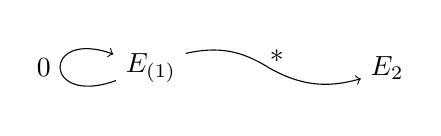
\begin{tikzpicture}
                        \node (e) at (0, 0) {$E_{(1)}$};
                        \node (e2) at (3, 0) {$E_2$};
                        \node () at (1.6, 0.1) {*};
                        \draw
                        (e) edge[out=200, in=160, distance=1cm, loop, left] node{0} (e)
                        (e) edge[bend left=22.5] (1.5, 0)
                        (1.5, 0) edge[->, bend right=22.5] (e2);
                    \end{tikzpicture}
                \end{center} 
                In the inductive case, we want to prove $P(k + 1)$, assuming $P(k)$.
                Because we're in a case where there's one or more steps, we can add a $E_1^\prime$ in our path, which is $k$ steps away from $E$.
                As we've assumed $P(k)$, it follows that there's some $E^{\prime\prime}$, such that $E_1^\prime \to^* E^{\prime\prime} \land E_2 \to^* E^{\prime\prime}$.
                This can be shown in the following diagram;
                \begin{center}
                    \begin{tikzpicture}[x=1.5cm, y=1.5cm]
                        \node (e) at (0, 0) {$E$};
                        \node (e1p) at (-1, -1) {$E_1^\prime$};
                        \node (e1) at (-2, -2) {$E_1$};
                        \node (e2) at (2, -2) {$E_2$};
                        \node (epp) at (0, -2) {$E^{\prime\prime}$};
                        \node () at (1.1, -0.9) {*};
                        \node () at (1.1, -1.9) {*};
                        \node () at (-0.4, -1.4) {*};
                        \draw
                        (e) edge[->, above] node{$k$} (e1p)
                        (e1p) edge[->] (e1)
                        (e) edge[bend right=22.5] (1, -1)
                        (1, -1) edge[->, bend left=22.5] (e2)
                        (e2) edge[bend left=22.5] (1, -2)
                        (1, -2) edge[->, bend right=22.5] (epp)
                        (e1p) edge[bend left=22.5] (-0.5, -1.5)
                        (-0.5, -1.5) edge[->, bend right=22.5] (epp);
                    \end{tikzpicture}
                \end{center}
                Now we can analyse the two cases;
                \begin{itemize}
                    \itemsep0em
                    \item $E_1^\prime = E^{\prime\prime}$
                        \subitem As we have $E_2 \to^* E^{\prime\prime}$, we get $E_2 \to^* E_1$, hence we can say $E^\prime = E_1$.
                    \item $E_1^\prime \neq E^{\prime\prime}$
                        \subitem
                            As they aren't the same, we can add a step in the path, hence $E_1^\prime \to E_1 \to^* E^{\prime\prime}$ ($E_1$ must be the next step due to determinacy).
                            Since we get $E_1 \to^* E^{\prime\prime}$, we can say $E^\prime = E^{\prime\prime}$.
                \end{itemize}
        \subsection*{30th October 2019 \hfill Lecture}
            \subsubsection*{SimpleExp}
                In this part of the lecture, our goal is to connect $\Downarrow$, and $\to^*$ for SimpleExp.
                Formally, we want to show;
                \begin{center}
                    $\forall E, n . E \Downarrow n \Leftrightarrow E \to^* n$
                \end{center}

                We first do the direction from $\Downarrow$ to $\to^*$, with the property $P(E) \triangleq \forall n . E \Downarrow n \Rightarrow E \to^* n$;
                \medskip

                There is almost no work to be done in the base case, where $E = n$, for some arbitrary $n \in \mathbb{N}$, as the big-step rule states that $n \Downarrow n$, and it takes 0 steps for $n$ to get to itself (in small-step).
                \smallskip

                For the inductive $+$ case, once again we are ignoring $\times$ as the results are quite similar, we take $E = E_1 + E_2$, with the inductive hypothesis $P(E_1) \land P(E_2)$.
                If we take some arbitrary $n$, such that $E \Downarrow n$, our rules for big-step require there to be some $n_1, n_2$ which satisfy $E_1 \Downarrow n_1$, $E_2 \Downarrow n_2$, and $n = n_1 + n_2$ (\textsc{b-add}).
                Additionally, due to our inductive hypothesis, we also get $E_1 \to^* n_1$, and also $E_2 \to^* n_2$.
                Since we have $E_1 \to^* n_1$, we can apply lemma 1, using (\textsc{s-left}), $r$ times, such that we have $E_1 + E_2 \to^* n_1 + E_2$.
                Similarly with lemma 2, using (\textsc{s-right}), we have $E_1 + E_2 \to^* n_1 + n_2$.
                Finally, due to (\textsc{s-add}), $E_1 + E_2 \to^* n$.
            \subsubsection*{While}
                In the second part of the lecture, we're revisiting the rules for the While language, which has the BNFs as follows;
                \begin{align*}
                    B \in \text{Bool} & ::= ~true~ \bnfsep ~false~ \bnfsep E = E \bnfsep E < E \bnfsep B \& B \bnfsep \neg B \bnfsep ... \\
                    E \in \text{Exp} & ::= x \bnfsep n \bnfsep E + E \bnfsep ... \\
                    C \in \text{Com} & ::= x := E \bnfsep ~if ~ B ~ then ~ C ~ else ~ C \bnfsep C;C \bnfsep ~skip~ \bnfsep ~while ~ B ~ do ~ C
                \end{align*}
                This has the following big-step rules;
                \begin{itemize}
                    \itemsep0em
                    \item \hfill
                            \axiom{$\la E, s \ra \Downarrow \la n, s^\prime \ra$}
                        \unary{$\la x := E, s \ra \Downarrow \la s^\prime [x \mapsto n] \ra$}
                        \dproof
                    \item \hfill
                            \axiom{$\la C_1, s \ra \Downarrow \la s^\prime \ra$}
                            \axiom{$\la C_2, s^\prime \ra \Downarrow \la s^{\prime\prime} \ra$}
                        \binary{$\la C_1; C_2, s \ra \Downarrow \la s^{\prime\prime} \ra$}
                        \dproof
                    \item \hfill
                            \axiom{$\la B, s \ra \Downarrow \la ~true~, s^\prime \ra$}
                            \axiom{$\la C_1, s^\prime \ra \Downarrow \la s^{\prime\prime} \ra$}
                        \binary{$\la ~if ~ B ~ then ~ C_1 ~ else ~ C_2, s \ra \Downarrow \la s^{\prime\prime} \ra$}
                        \dproof
                    \item \hfill
                            \axiom{$\la B, s \ra \Downarrow \la ~false~, s^\prime \ra$}
                            \axiom{$\la C_2, s^\prime \ra \Downarrow \la s^{\prime\prime} \ra$}
                        \binary{$\la ~if ~ B ~ then ~ C_1 ~ else ~ C_2, s \ra \Downarrow \la s^{\prime\prime} \ra$}
                        \dproof
                    \item \hfill
                            \axiom{$\la B, s \ra \Downarrow \la ~true~, s^\prime \ra$}
                            \axiom{$\la C, s^\prime \ra \Downarrow \la s^{\prime\prime} \ra$}
                            \axiom{$\la ~while ~ B ~ do ~ C, s^{\prime\prime} \Downarrow \la s^{\prime\prime\prime} \ra$}
                        \trinary{$\la ~while ~ B ~ do ~ C, s \ra \Downarrow \la s^{\prime\prime\prime} \ra$}
                        \dproof
                    \item \hfill
                            \axiom{$\la B, s \ra \Downarrow \la ~false~, s^\prime \ra$}
                        \unary{$\la ~while ~ B ~ do ~ C, s \ra \Downarrow \la s^\prime \ra$}
                        \dproof
                \end{itemize}
            After this point, there isn't any sound on the Panopto recording; the remainder of the lecture goes over heaps found in the coursework.
        \subsection*{6th November 2019 \hfill Tutorial}
            The lecture starts off going over questions in the coursework.
            Note that the question concerning $\neg$ can be done in a single case, with a side condition;
            \begin{center}
                    \axiom{$\la B, s, h \ra \Downarrow \la b, s^\prime, h^\prime \ra$}
                \unary{$\la \neg B, s, h \ra \Downarrow \la b^\prime, s^\prime, h^\prime \ra$}
                \dproof
                \violet{$b^\prime = \neg b$}
            \end{center}
            The next part concerns question 1 from last year's exam, which involves the language \textsc{ForWithBreak};
            \begin{align*}
                C & ::= ~skip~ \bnfsep ~break~ \bnfsep x := E \bnfsep ~if ~ B ~ then ~ C ~ else ~ C \bnfsep ~for ~ x ~ in ~ [E, E] ~ do ~ C \bnfsep C ; C \\
                \mathcal{O} & ::= \mathcal{N} \bnfsep \mathcal{B}
            \end{align*}
            Writing out the big-step rules is too much effort; refer to the exam paper for the trees.
            \bigskip

            The ~for~ loop iterates between the values in the range, substituting $x$ for each of the values iteratively, to be used in $C$.
            The way ~break~ works is by terminating sequential commands; for example, if we had $C = ~break~; C_2$, it would evaluate to $\mathcal{B}$, and skipping the execution of $C_2$.
            However, if a ~break~ is encountered within a ~for~ loop, such that $\la C, s \ra \Downarrow_c \la \mathcal{B}, s^\prime \ra$, we terminate the loop, and then the program continues normally, such that the loop command evaluates to $\la \mathcal{N}, s^\prime \ra$.
        \subsection*{7th November 2019 \hfill Lecture}
            \subsubsection*{Register Machines}
                In a register machine, we operate on registers with idealised natural numbers (hence we don't consider physical limitations such as overflow).
                The elementary operations available to us are as follows;
                \begin{itemize}
                    \itemsep0em
                    \item add 1 to a register
                    \item jumps
                    \item test whether a register is 0 (+ conditionals)
                    \item subtract 1 from a non-zero register
                \end{itemize}
                Formally, a register machine is specified with finitely many registers ($R_0, R_1, \dots, R_n$), and a finite list of instructions, of the following form;
                \begin{center}
                    \begin{tabular}{|l|l|}
                        \hline
                        label: body & description \\
                        \hline
                        $L_i: R^+ \to L^\prime$ & Add 1 to the contents of $R$, and jump to $L^\prime$ \\
                        $L_i: R^- \to L^\prime, L^{\prime\prime}$ & If $R > 0$, subtract 1 from $R$, and jump to $L^\prime$, else jump to $L^{\prime\prime}$ \\
                        ~HALT~ & Terminate the program \\
                        \hline
                    \end{tabular}
                \end{center}
                A register machine's configuration is written in the following form;
                \begin{center}
                    $c = (\ell, r_0, \dots, r_n)$
                \end{center}
                We define a computation of a register machine as a sequence of configurations; $c_0, c_1, \dots$, where $c_0$ is the initial configuration, and $c_{i + 1}$ is determined by the previous ($c_i$) configuration.
                This sequence \textbf{can} be infinite, if the program does not halt.
                A program halts if it reaches the ~HALT~ instruction (a \textbf{proper} halt), or there is a jump to an instruction that does not exist (an \textbf{erroneous} halt).
            \subsubsection*{Graphical Representation}
                We can also represent these instructions graphically, instead of as a list of instructions.
                Note that $[L]$ means the body of the instruction with label $L$.
                \begin{center}
                    \begin{tabular}{|l|c|}
                        \hline
                        instruction & representation \\
                        \hline
                        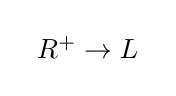
\begin{tikzpicture}
                            \node () at (0, 0) {$R^+ \to L$};
                        \end{tikzpicture} &
                        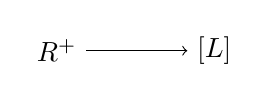
\begin{tikzpicture}
                            \node (r) at (0, 0) {$R^+$};
                            \node (l) at (2, 0) {$[L]$};
                            \draw
                            (r) edge[->] (l);
                        \end{tikzpicture} \\
                        \hline
                        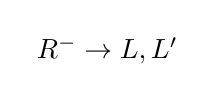
\begin{tikzpicture}
                            \node () at (0, 0) {$R^- \to L, L^\prime$};
                        \end{tikzpicture} &
                        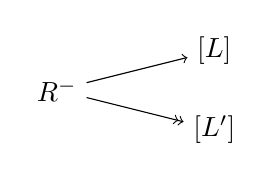
\begin{tikzpicture}
                            \node (r) at (0, 0) {$R^-$};
                            \node (l) at (2, 0.5) {$[L]$};
                            \node (lp) at (2, -0.5) {$[L^\prime]$};
                            \draw
                            (r) edge[->] (l)
                            (r) edge[->>] (lp);
                        \end{tikzpicture} \\
                        \hline
                    \end{tabular}
                \end{center}
            \subsubsection*{Partial Functions}
                We define a partial function from a set $X$ to a set $Y$, as any subset $f \subseteq X \times Y$, such that $(x, y) \in f \land (x, y^\prime) \in f \Rightarrow y = y^\prime$.
                \smallskip

                Additional notation is as follows;
                \begin{itemize}
                    \itemsep0em
                    \item $f(x) = y$ \hfill $(x, y) \in f$
                    \item $f(x) \downarrow$ \hfill $\exists y \in Y . [f(x) = y]$
                        \subitem $x$ maps to something in $y$, under $f$
                    \item $f(x) \uparrow$ \hfill $\neg \exists y \in Y . [f(x) = y]$
                        \subitem $x$ doesn't map to something in $y$, under $f$
                    \item $X \rightharpoonup Y$ is the set of all \textbf{partial} functions from $X$ to $Y$, whereas $X \to Y$ is the set of all \textbf{total} functions
                        \subitem a partial function $f$ is total if $\forall x \in X . [f(x) \downarrow]$
                \end{itemize}
                We define a function $f \in \mathbb{N}^n \rightharpoonup \mathbb{N}$ as computable if there is a register machine with at least $n + 1$ registers such that for all $(x_1, \dots, x_n) \in \mathbb{N}^n$, starting at the configuration $c = (0, 0, x_1, \dots, x_n, 0, \dots, 0)$ halts with $R_0 = y$ if and only if $f(x_1, \dots, x_n) = y$.
                \medskip

                Register machines can be constructed to prove the computability of functions.
                For example, multiplication can be done with an auxiliary register; every time $x$ is reduced by 1, $y$ is copied into the auxiliary register, as well as $R_0$, and then $y$ is restored from the auxiliary register.
        \subsection*{13th November 2019 \hfill Lecture}
            \subsubsection*{Numerical Coding of Pairs}
                The goal is to get a bijection between pairs of natural numbers, and the natural numbers themselves, for example the representation gives us the equivalence $27 = ~0b11011~ = \lla 0, 13 \rra = \la 2, 3 \ra$;
                \begin{align*}
                    \lla x, y \rra & \triangleq 2^x (2y + 1) & \text{bijection between } \mathbb{N} \times \mathbb{N} \text{ and } \mathbb{N}^+ \\
                    \la x, y \ra & \triangleq 2^x (2y + 1) - 1 & \text{bijection between } \mathbb{N} \times \mathbb{N} \text{ and } \mathbb{N}
                \end{align*}
                We can convert $\lla x, y \rra$ to binary as first $y$ in binary, followed by a ~1~, and then followed by $x$ ~0~s, as we shift it by $x$ bits.
                Similarly, $\la x, y \ra$ can be thought of as $y$ in binary, followed by a ~0~, and then $x$ ~1~s (since we can subtract ~1~ from ~1~ and $x$ ~0~s).
            \subsubsection*{Numerical Coding of Lists}
                $List\ \mathbb{N}$ is defined as the set of all finite lists of natural numbers, with the following rules;
                \begin{itemize}
                    \itemsep0em
                    \item the empty list: \hfill $[] \in List\ \mathbb{N}$
                    \item the cons list: \hfill $x \in \mathbb{N} \land \ell \in List\ \mathbb{N} \Rightarrow x :: \ell \in List\ \mathbb{N}$
                    \item shorthand notation: \hfill $[x_1, x_2, \dots, x_n] \triangleq x_1 :: (x_2 :: (\dots :: (x_n :: []) \dots )$
                \end{itemize}
                Our notation will use $\crnr{\ell} \in \mathbb{N}$ to represent the natural number representing the list $\ell \in List\ \mathbb{N}$;
                \begin{align*}
                    \crnr{[]} & \triangleq 0 \\
                    \crnr{x :: \ell} & \triangleq \lla x, \crnr{\ell} \rra = 2^x (2 \cdot \crnr{\ell} + 1)
                \end{align*}
                Therefore, we can say $\crnr{[x_1, x_2, \dots, x_n]} = \lla x_1, \lla x_2, \lla \dots \lla x_n, 0 \rra \dots \rra \rra \rra$
                \medskip

                We can also obtain the following result;
                \begin{center}
                    ~0b~$\crnr{[x_1, x_2, \dots, x_n]} = ~1~\underbrace{~0~\cdots~0~}_\text{$x_n$ ~0~s}~1~\underbrace{~0~\cdots~0~}_\text{$x_{n-1}$ ~0~s} \cdots ~1~\underbrace{~0~\cdots~0~}_\text{$x_1$ ~0~s}$
                \end{center}
            \subsubsection*{Numerical Coding of Programs}
                Consider some register machine program $P$;
                \begin{align*}
                    L_0 & : b_0 \\
                    L_1 & : b_1 \\
                    \vdots \\
                    L_n & : b_n
                \end{align*}
                The program's encoding is $\crnr{P} \triangleq \crnr{[\crnr{b_0}, \crnr{b_1}, \dots, \crnr{b_n}]}$.
                The bodies can be encoded as such;
                \begin{align*}
                    \crnr{R_i^+ \to L_j} & \triangleq \lla 2i, j \rra \\
                    \crnr{R_i^- \to L_j, L_k} & \triangleq \lla 2i + 1, \la j, k \ra \rra \\
                    \crnr{~HALT~} & \triangleq 0
                \end{align*}
        \subsection*{14th November 2019 \hfill Lecture}
            \subsubsection*{Gadgets}
                We can think of these building blocks as subroutines.
                These gadgets have one entry point, but can have multiple exit points.
                These gadgets can use scratch registers, assuming they are initialised to 0, but must reset them back to 0 after execution.
                Gadgets can also use other registers (however they must be specified), and we can use them to contain arguments to the gadgets, the start initialisation of the gadget, or the result of what the gadget is producing.
                \medskip

                Here are some examples of gadgets, and their graphical representations;
                \begin{itemize}
                    \itemsep0em
                    \item zero $R_n$ \hfill $R_n = 0$
                        \begin{center}
                            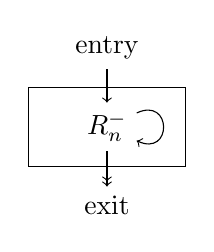
\begin{tikzpicture}[y=0.5cm]
                                \node (en) at (0, 0) {entry};
                                \node (ex) at (0, -4) {exit};
                                \node (r) at (0, -2) {$R_n^-$};
                                \draw
                                (en) edge[->] (r)
                                (r) edge[->, loop, out=25, in=-25, distance=0.5cm] (r)
                                (r) edge[->>] (ex)
                                (-1, -1) -- (1, -1) -- (1, -3) -- (-1, -3) -- cycle;
                            \end{tikzpicture}
                        \end{center}
                    \item add $R_i$ to $R_j$ \hfill $R_j = R_j + R_i$
                        \begin{center}
                            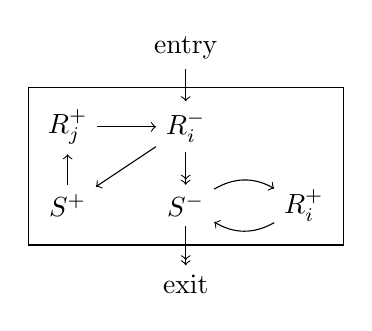
\begin{tikzpicture}[y=0.5cm]
                                \node (en) at (0, 0) {entry};
                                \node (ex) at (0, -6) {exit};
                                \node (rim) at (0, -2) {$R_i^-$};
                                \node (sm) at (0, -4) {$S^-$};
                                \node (sp) at (-1.5, -4) {$S^+$};
                                \node (rjp) at (-1.5, -2) {$R_j^+$};
                                \node (rip) at (1.5, -4) {$R_i^+$};
                                \draw
                                (en) edge[->] (rim)
                                (rim) edge[->>] (sm)
                                (sm) edge[->>] (ex)
                                (rim) edge[->] (sp)
                                (sp) edge[->] (rjp)
                                (rjp) edge[->] (rim)
                                (sm) edge[->, bend left=30] (rip)
                                (rip) edge[->, bend left=30] (sm)
                                (-2, -1) -- (2, -1) -- (2, -5) -- (-2, -5) -- cycle;
                            \end{tikzpicture}
                        \end{center}
                \end{itemize}
                With these gadgets, we can then chain them to produce other gadgets.
                For example, we can copy the value of $R_i$ into $R_j$ (such that $R_j$'s old value is replaced with $R_i$'s), by first zeroing $R_j$ with the first gadget, and then adding $R_i$ to it, with the second gadget.
                \smallskip

                Another important gadget is one to perform the push operation, which essentially performs $x :: \ell$.
                The following gadget pushes $X$ to $L$, such that $X = x, L = \ell, X^\prime = 0, L^\prime = \lla x, \ell \rra = 2^x (2 \ell + 1)$, where $X^\prime$ and $L^\prime$ are the values of $X$ and $L$ after the gadget, respectively.
                These work with the numerical coding of lists.
                The proof for this is in the notes, in \textit{Lecture 6 - Universal RM.pdf}.
                \begin{center}
                    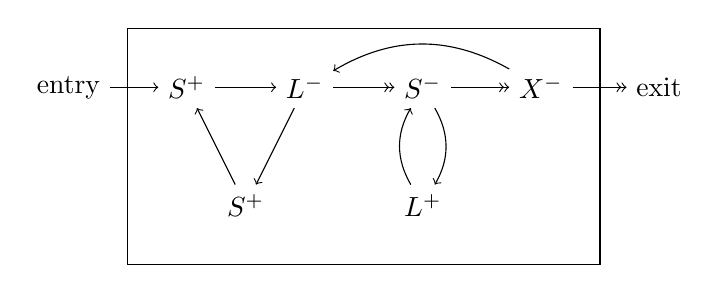
\begin{tikzpicture}[x=1.5cm, y=1.5cm]
                        \node (en) at (0, 0) {entry};
                        \node (sp1) at (1, 0) {$S^+$};
                        \node (lm) at (2, 0) {$L^-$};
                        \node (sm) at (3, 0) {$S^-$};
                        \node (xm) at (4, 0) {$X^-$};
                        \node (ex) at (5, 0) {exit};
                        \node (sp2) at (1.5, -1) {$S^+$};
                        \node (lp) at (3, -1) {$L^+$};
                        \draw
                        (en) edge[->] (sp1)
                        (sp1) edge[->] (lm)
                        (lm) edge[->] (sp2)
                        (sp2) edge[->] (sp1)
                        (lm) edge[->>] (sm)
                        (sm) edge[->>] (xm)
                        (xm) edge[->>] (ex)
                        (xm) edge[->, bend right=30] (lm)
                        (sm) edge[->, bend left=30] (lp)
                        (lp) edge[->, bend left=30] (sm)
                        (0.5, 0.5) -- (4.5, 0.5) -- (4.5, -1.5) -- (0.5, -1.5) -- cycle;
                    \end{tikzpicture}
                \end{center}
        \subsection*{20th November 2019 \hfill Lecture}
            Continuing on from last week's lecture, we look at the gadget to perform the pop operation, which has two outcomes.
            In the first outcome, where the list is empty $L = \ell = 0$, then we return with $X^\prime = 0$.
            On the other hand, we return $X^\prime = x$, and $L^\prime = \ell$, if the initial state is $L = \lla x, \ell \rra$.
            \begin{center}
                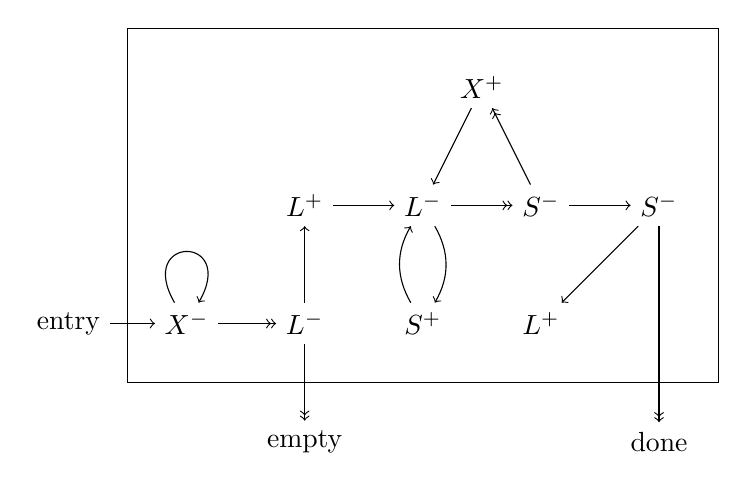
\begin{tikzpicture}[x=1.5cm, y=1.5cm]
                    \node (en) at (0, 0) {entry};
                    \node (xm) at (1, 0) {$X^-$};
                    \node (lm1) at (2, 0) {$L^-$};
                    \node (lp1) at (2, 1) {$L^+$};
                    \node (lm2) at (3, 1) {$L^-$};
                    \node (sp) at (3, 0) {$S^+$};
                    \node (sm1) at (4, 1) {$S^-$};
                    \node (sm2) at (5, 1) {$S^-$};
                    \node (lp2) at (4, 0) {$L^+$};
                    \node (xp) at (3.5, 2) {$X^+$};
                    \node (em) at (2, -1) {empty};
                    \node (do) at (5, -1) {done};
                    \draw
                    (en) edge[->] (xm)
                    (xm) edge[->, loop, out=120, in=60, distance=1cm] (xm)
                    (xm) edge[->>] (lm1)
                    (lm1) edge[->>] (em)
                    (lm1) edge[->] (lp1)
                    (lp1) edge[->] (lm2)
                    (lm2) edge[->>] (sm1)
                    (sm1) edge[->] (sm2)
                    (sm2) edge[->] (lp2)
                    (sm2) edge[->>] (do)
                    (sm1) edge[->>] (xp)
                    (xp) edge[->] (lm2)
                    (lm2) edge[->, bend left=30] (sp)
                    (sp) edge[->, bend left=30] (lm2)
                    (0.5, 2.5) -- (5.5, 2.5) -- (5.5, -0.5) -- (0.5, -0.5) -- cycle;
                \end{tikzpicture}
            \end{center}
            \subsubsection*{The Universal Register Machine}
                This gadgets used in the universal register machine are \textbf{copy}, \textbf{push}, and \textbf{pop}.
                The universal register machine is an interpreter of the Godel number of programs.
                It starts with $R_0 = 0$, which is designed to be the return value of the program, $R_1 = e = \crnr{P}$ (the code of a program), and $R_2 = a = \crnr{[a_1, \dots, a_n]}$ (a list of arguments).
                The goal of the universal register machine is to carry out the computation of $P$ starting with $R_0 = 0, R_1 = a_1, \dots R_n = a_n$, and all other registers at 0.
                The mnemonics of the registers in $U$ are as follows (anything else can be used as a scratch register);
                \begin{enumerate}[${R}_1 \equiv$]
                    \itemsep0em
                    \setcounter{enumi}{-1}
                    \item ??? \hfill result of simulated computation (if any)
                    \item $P$ \hfill \textbf{p}rogram code of the register machine to be simulated
                    \item $A$ \hfill list of \textbf{a}rguments / register contents of the simulated machine
                    \item $PC$ \hfill \textbf{p}rogram \textbf{counter} - current instruction label
                    \item $N$ \hfill label number(s) of the \textbf{n}ext instruction(s), also code for current instruction
                    \item $C$ \hfill code of the \textbf{c}urrent instruction body
                    \item $R$ \hfill value of the \textbf{r}egister to be used by current instruction
                    \item $S$ \hfill auxiliary register
                    \item $T$ \hfill auxiliary register
                \end{enumerate}
                The overall execution structure of the universal register machine is as follows;
                \begin{enumerate}[1.]
                    \itemsep0em
                    \item copy $PC^\text{th}$ instruction of $P$ to $N$ (halt if $PC > \text{length of list}$), and go to step 2.
                    \item if $N = 0$, then halt, otherwise $N = \lla y, z \rra$, then set $C = y, N = z$, and go to step 3.
                        \subitem if $C = 2i$ then instruction is $R_i^+ \to L_z$
                        \subitem if $C = 2i + 1$ then instruction is $R_i^- \to L_j, L_k$, where $z = \la j, k \ra$
                        \subitem note that in this case, when we say $R_i$, we're referring to the register in the \textbf{simulated} machine not the \textbf{universal} machine.
                    \item copy $i^\text{th}$ item of $A$ to $R$, and go to step 4
                    \item execute the current instruction on $R$, update the $PC$ to the next label, restore the register value to $A$, and go to step 1
                \end{enumerate}
                The universal register machine can be represented graphically as below.
                For a full explanation of how the steps work in detail, the lecture explains it well.
                Note that the single $N^+$ converts between the single and double angle encodings, since the single angle encoding is used for $\la j, k \ra$.
                \begin{center}
                    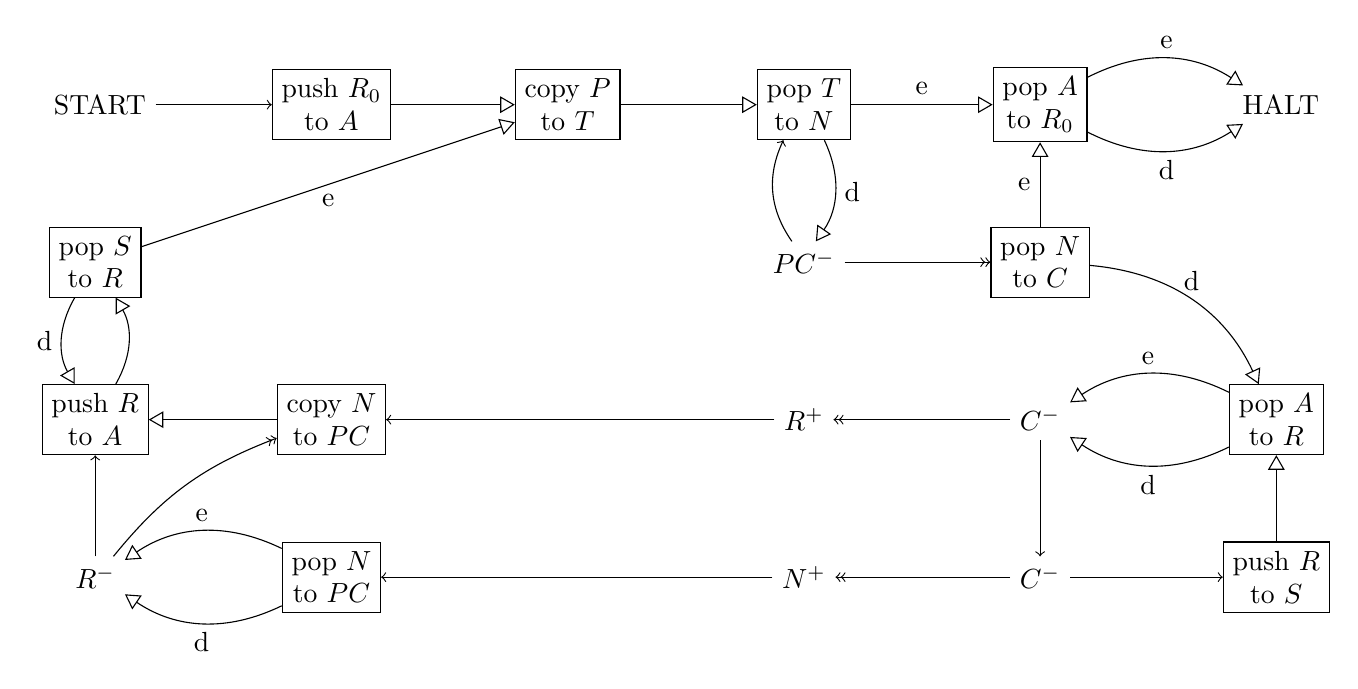
\begin{tikzpicture}[x=3cm, y=2cm]
                        \node (s) at (0, 0) {~START~};
                        \node[draw] (pur0a) at (1, 0) {\shortstack{push $R_0$ \\ to $A$}};
                        \node[draw] (copt) at (2, 0) {\shortstack{copy $P$ \\ to $T$}};
                        \node[draw] (potn) at (3, 0) {\shortstack{pop $T$ \\ to $N$}};
                        \node[draw] (poar0) at (4, 0) {\shortstack{pop $A$ \\ to $R_0$}};
                        \node (h) at (5, 0) {~HALT~};
                        \node[draw] (posr) at (0, -1) {\shortstack{pop $S$ \\ to $R$}};
                        \node (pcm) at (3, -1) {$PC^-$};
                        \node[draw] (ponc) at (4, -1) {\shortstack{pop $N$ \\ to $C$}};
                        \node[draw] (pura) at (0, -2) {\shortstack{push $R$ \\ to $A$}};
                        \node[draw] (conpc) at (1, -2) {\shortstack{copy $N$ \\ to $PC$}};
                        \node (rp) at (3, -2) {$R^+$};
                        \node (cm1) at (4, -2) {$C^-$};
                        \node[draw] (poar) at (5, -2) {\shortstack{pop $A$ \\ to $R$}};
                        \node (rm) at (0, -3) {$R^-$};
                        \node[draw] (ponpc) at (1, -3) {\shortstack{pop $N$ \\ to $PC$}};
                        \node (np) at (3, -3) {$N^+$};
                        \node (cm2) at (4, -3) {$C^-$};
                        \node[draw] (purs) at (5, -3) {\shortstack{push $R$ \\ to $S$}};
                        \draw
                        (s) edge[->] (pur0a)
                        (pur0a) edge[-{open triangle 60}] (copt)
                        (copt) edge[-{open triangle 60}] (potn)
                        (potn) edge[-{open triangle 60}, above] node{e} (poar0)
                        (poar0) edge[-{open triangle 60}, bend left=30, above] node{e} (h)
                        (poar0) edge[-{open triangle 60}, bend right=30, below] node{d} (h)
                        (posr) edge[-{open triangle 60}, below] node{e} (copt)
                        (pcm) edge[->, bend left=30] (potn)
                        (potn) edge[-{open triangle 60}, bend left=30, right] node{d} (pcm)
                        (ponc) edge[-{open triangle 60}, left] node{e} (poar0)
                        (pcm) edge[->>] (ponc)
                        (posr) edge[-{open triangle 60}, bend right=30, left] node{d} (pura)
                        (pura) edge[-{open triangle 60}, bend right=30] (posr)
                        (ponc) edge[-{open triangle 60}, bend left=30, above] node{d} (poar)
                        (conpc) edge[-{open triangle 60}] (pura)
                        (rp) edge[->] (conpc)
                        (cm1) edge[->>] (rp)
                        (poar) edge[-{open triangle 60}, bend right=30, above] node{e} (cm1)
                        (poar) edge[-{open triangle 60}, bend left=30, below] node{d} (cm1)
                        (rm) edge[->] (pura)
                        (rm) edge[->>, bend left=15] (conpc)
                        (cm1) edge[->] (cm2)
                        (purs) edge[-{open triangle 60}] (poar)
                        (ponpc) edge[-{open triangle 60}, bend right=30, above] node{e} (rm)
                        (ponpc) edge[-{open triangle 60}, bend left=30, below] node{d} (rm)
                        (np) edge[->] (ponpc)
                        (cm2) edge[->>] (np)
                        (cm2) edge[->] (purs);
                    \end{tikzpicture}
                \end{center}
            \subsubsection*{Halting Problem}
                We define a register machine $H$ to decide the Halting Problem, if for all $e, a_1, \dots, a_n \in \mathbb{N}$, starting $H$ with the configuration $(\ell, 0, e, \crnr{[a_1, \dots, a_n]})$ (where $\ell$ is some starting label), the computation of $H$ always halts with $R_0 = 0$ or $1$.
                $R_0 = 1$ iff the register machine with index $e$ eventually halts with $R_0 = 0, R_1 = a_1, \dots, R_n = a_n$.
                Clearly, simulation doesn't work; if the program with index $e$ doesn't halt, then $H$ cannot halt if it simulates it.
                \medskip

                We can prove this machine cannot exist by contradiction.
                Let us first add two steps, after the program starts - we name this new machine $H^\prime$;
                \begin{enumerate}[1.]
                    \itemsep0em
                    \item $Z = R_1$ \hfill $Z$ is some unused register
                    \item push $Z$ to $R_2$ \hfill adding the program as an argument
                \end{enumerate}
                Then, every normal ~HALT~ or erroneous halt is replaced with the following loop;
                \begin{center}
                    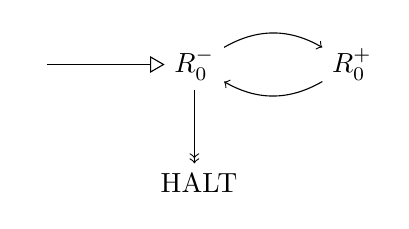
\begin{tikzpicture}[x=2cm, y=1.5cm]
                        \node (s) at (0, 0) {};
                        \node (r0m) at (1, 0) {$R_0^-$};
                        \node (r0p) at (2, 0) {$R_0^+$};
                        \node (h) at (1, -1) {~HALT~};
                        \draw
                        (s) edge[-{open triangle 60}] (r0m)
                        (r0m) edge[->, bend left=30] (r0p)
                        (r0p) edge[->, bend left=30] (r0m)
                        (r0m) edge[->>] (h);
                    \end{tikzpicture}
                \end{center}
                Let us now call this new register machine, based off of $H^\prime$, $C$, with program index $c \in \mathbb{N}$.
                \medskip

                As such, $C$ starting with $R_1 = c$ eventually halts iff $H^\prime$ starting with $R_1 = c$ halts with $R_0 = 0$ iff $H$ starting with $R_1 = c, R_2 = \crnr{[c]}$ halts with $R_0$ iff $C$ starting with $R_1 = c$ does not halt.
        \subsection*{21st November 2019 \hfill Lecture}
            For each $e \in \mathbb{N}$, let $\phi_e \in \mathbb{N} \rightharpoonup \mathbb{N}$ be the partial function computed by the register machine with index $e$. $\phi_e(x) = y$ holds iff the register machine halts with $R_0 = y$, after starting with $R_0 = 0, R_1 = x$.
            \medskip

            Let $f \in \mathbb{N} \rightharpoonup \mathbb{N}$ be the partial function $\{(x, 0) \bnfsep \phi_x(x) \uparrow\}$, such that
            \begin{align*}
                f(x) & =
                \begin{cases}
                    0 & \text{if } \phi_x(x) \uparrow \text{ (uncomputable)} \\
                    \text{undefined} & \text{if } \phi_x(x) \downarrow \text{ (computable)}
                \end{cases}
            \end{align*}
            If we assume that $f$ is computable, then $f = \phi_e$, for some $e \in \mathbb{N}$.
            We can consider each case;
            \begin{itemize}
                \itemsep0em
                \item $\phi_e(e) \uparrow$, then $f(e) = 0$, by definition of $f$, which therefore means $f\phi_e(e) = 0$, but then it is computable hence $\phi_e(e) \downarrow$
                \item $\phi_e(e) \downarrow$, then $f(e) = \text{undefined}$, hence $\phi_e(e) \uparrow$
            \end{itemize}
            As both cases lead to a contradiction, the entire assumption fails, hence $f$ isn't computable.
            \medskip

            A similar application can be done to sets; take a subset $S \subseteq \mathbb{N}$, the \textbf{characteristic function} of $S$, $\chi_S \in \mathbb{N} \to \mathbb{N}$, is defined as follows;
            \begin{align*}
                \chi_S(x) & =
                \begin{cases}
                    1 & \text{if } x \in S \\
                    0 & \text{if } x \notin S
                \end{cases}
            \end{align*}
            A subset $S$ is called RM decidable if its characteristic function $\chi_S$ is a register machine computable function.
            Therefore, $S$ is decidable if there is some register machine $M$ such that for all $x \in \mathbb{N}$, $M$ eventually terminates with $R_0 = \chi_S(x)$, when starting with $R_0 = 0, R_1 = 1$.
            \subsubsection*{Turing Machines}
                Informally a Turing machine is a head with a state, on a tape with symbols.
                It has the following characteristics;
                \begin{itemize}
                    \itemsep0em
                    \item the machine starts in state $s$ with the tape head pointing to the first symbol of the finite input string (everything else is blank)
                    \item the machine computes in steps, depending on the current state of the head, and the symbol being scanned by the tape head
                    \item an action is to overwrite the current tape cell with a symbol, move left or right one cell, and change state
                    \item finitely many states
                    \item finitely many symbols
                \end{itemize}
                Formally, a Turing machine is specified by a quadruple $M = (Q, \Sigma, s, \delta)$, where;
                \begin{itemize}
                    \itemsep0em
                    \item $Q$ \hfill a finite set of machine states
                    \item $\Sigma$ \hfill a finite set of tape symbols (containing a \textbf{blank} - \textvisiblespace)
                    \item $s \in Q$ \hfill an initial state
                    \item $\delta \in (Q \times \Sigma) \rightharpoonup (Q \times \Sigma \times \{L, R\})$ \hfill a partial transition function
                        \subitem this takes the current state, the current symbol, and possibly creates the next state, the next symbol, and a movement to the left or right
                        \subitem note that it is a partial function; if it reaches something it cannot do, the machine halts
                \end{itemize}
                We can then formally define a configuration $(q, w, u)$ as;
                \begin{itemize}
                    \itemsep0em
                    \item $q \in Q$ \hfill the current state
                    \item $w \in \Sigma^*$ \hfill a finite (possibly empty) string of tape symbols to the left of the head
                    \item $u \in \Sigma^*$ \hfill a finite (possibly empty) string of tape symbols under and to the right of the head
                \end{itemize}
                An initial configuration is $(s, \epsilon, u)$, for an initial state, and a string of tape symbols $u$.
                \medskip

                We can define elementary functions $\text{first} : \Sigma^* \to \Sigma \times \Sigma^*$, and $\text{last} : \Sigma^* \to \Sigma \times \Sigma^*$ as follows, which split off the first and last symbols of a string.
                \begin{align*}
                    \text{first}(w) & =
                    \begin{cases}
                        (a, v) & \text{if } w = a v \\
                        (\text{\textvisiblespace}, \epsilon) & \text{if } w = \epsilon \\
                    \end{cases} \\
                    \text{last}(w) & =
                    \begin{cases}
                        (a, v) & \text{if } w = v a \\
                        (\text{\textvisiblespace}, \epsilon) & \text{if } w = \epsilon \\
                    \end{cases}
                \end{align*}
                From this, we can define the computation of a Turing Machine $M = (Q, \Sigma, s, \delta)$, $(q, w, u) \to_M (q^\prime, w^\prime, u^\prime)$ by;
                \begin{itemize}
                    \item
                            \axiom{$\text{first}(u) = (a, u^\prime)$}
                            \axiom{$\delta(q, a) = (q^\prime, a^\prime, L)$}
                            \axiom{$\text{last}(w) = (b, w^\prime)$}
                        \trinary{$(q, w, u) \to_M (q^\prime, w^\prime, b a^\prime u^\prime)$}
                        \dproof
                    \item
                            \axiom{$\text{first}(u) = (a, u^\prime)$}
                            \axiom{$\delta(q, a) = (q^\prime, a^\prime, R)$}
                        \binary{$(q, w, u) \to_M (q^\prime, w a^\prime, u^\prime)$}
                        \dproof
                \end{itemize}
                If $(q, w, u)$ has no computation step, it is a \textbf{normal form}, this happens when $\delta(q, a)$ isn't defined for $\text{first}(u) = (a, u^\prime)$.
                The computation for a Turing Machine $M$ is a sequence of configurations $c_0, c_1, c_2, \dots$, where $c_0 = (s, \epsilon, u)$ is an initial configuration, and $c_i \to_M c_{i + 1}$ holds for all $i$. This computation does not halt if the sequence is infinite, but does halt if the sequence is finite and the last element is a normal form.
        \subsection*{27th November 2019 \hfill Lecture}
            \subsubsection*{The $\lambda$-Calculus}
                This can be considered the "simplest programming language", where it is defined as follows;
                \begin{center}
                    $\violet{M} ::= x \bnfsep \lambda x.\ \violet{M} \bnfsep \violet{M}\ \violet{M}$
                \end{center}
                \begin{itemize}
                    \itemsep0em
                    \item $x$ \hfill a variable
                    \item $\lambda x . \violet{M}$ \hfill an abstraction (single-parameter function, where $\violet{M}$ is the body)
                    \item $\violet{M}\ \violet{M}$ \hfill an application
                \end{itemize}
                For example, $\lambda x.\ (2x + 1)$ is equivalent to ~x => 2*x + 1~ in Scala.
            \subsubsection*{Syntax}
                A variable is bound in $\violet{M}$ if it has a corresponding $\lambda$ (binder), for example (bound variables in \red{red}, free variables in \blue{blue});
                \begin{itemize}
                    \itemsep0em
                    \item $\lambda x.\ \red{x}$
                    \item $\lambda x.\ \blue{y}$
                    \item $\lambda x.\ \lambda y.\ \lambda z.\ \red{x} \red{y} $ \hfill with \textbf{contraction}, it can also be written as $\lambda xyz.\ \red{x} \red{y}$
                    \item $((\lambda x.\ \red{x} \blue{y})(\lambda y.\ \blue{x} \red{y}))(\lambda xy.\ \red{x} \red{y} \blue{z})$ \hfill application is \textbf{left-associative}
                    \item $(\lambda x.\ (\lambda y.\ \red{x} \red{y}) \blue{y})(\lambda z.\ \red{z} \blue{x})$
                \end{itemize}
                A \textbf{closed term} has no free variables.
                Formally, we can define free variables on the structure of $\violet{M}$ as follows;
                \begin{align*}
                    \text{FV}(x) & = \{x\} & \text{all variables are free by themselves} \\
                    \text{FV}(\lambda x.\ \violet{M}) & = \text{FV}(\violet{M}) \setminus \{x\} \\
                    \text{FV}(\violet{M} \violet{N}) & = \text{FV}(\violet{M}) \cup \text{FV}(\violet{N})
                \end{align*}
                In terms of programming languages, we can consider bound variables as function parameters.
                \begin{lstlisting}
                    function (x, y) {
                        return x + y;
                    }
                \end{lstlisting}
                Can be written as $\lambda xy.\ x + y$ (assuming we had some sort of arithmetic plus operator).
                On the other hand, free variables are "declared" in a higher-up scope, for example;
                \begin{lstlisting}
                    function (x, y) {
                        return (x + y) % z;
                    }
                \end{lstlisting}
            \subsubsection*{Tutorial}
                \begin{enumerate}[(a)]
                    \itemsep0em
                    \item Doing this as one question; the colours are as follows; \violet{binding occurrences}, \red{bound occurrences}, and \blue{free occurrences};
                        \medskip

                        $(\lambda \violet{x} \violet{y}.\ \red{y} (\lambda \violet{x}.\ \red{x} \red{y}) \blue{z})(\blue{x}(\lambda \violet{z} \violet{x}.\ \red{x} \red{z} \blue{y}))$
                    \item Not really bothered to write this out, the main point is to consider scoping.
                \end{enumerate}
            \subsubsection*{$\alpha$-equivalence}
                The process of renaming bound variables is called $\alpha$-equivalence.
                Syntactically, the functions on lines 1 and 2 are different, but they are semantically the same;
                \begin{lstlisting}
                    function(x, y) { return x + y; }
                    function(a, b) { return a + b; }
                \end{lstlisting}
                The functions can be represented as the following $\lambda$-terms, omitting the plus; $\lambda xy.\ x y$ and $\lambda ab.\ a b$ respectively.
                In the $\lambda$-calculus, they are the same, despite being represented differently, they are computed the same, therefore;
                \begin{center}
                    $\lambda xy.\ x y =_\alpha \lambda ab.\ a b$
                \end{center}
                Intuitively, $\violet{M} =_\alpha \violet{N}$ iff one can be obtained from the other (obviously both ways) by reaming the bound variables.
                They must also have the same set of free variables.
                The general strategy is as follows;
                \begin{itemize}
                    \itemsep0em
                    \item Are they of the same structure?
                    \item Do all of the free variables match?
                    \item Can you rename the bound variables so that they match?
                \end{itemize}
            \subsubsection*{Substitution}
                In the $\lambda$-calculus, we use the syntax $M[N / x]$, to replace $x$ with $N$ in $M$.
                \begin{itemize}
                    \itemsep0em
                    \item $x[y / x]$ \hfill $y$
                        \subitem the $x$ is replaced with a $y$
                    \item $z[y / x]$ \hfill $z$
                        \subitem there is no $x$ to replace
                    \item $(x y)(y z)[y / x]$ \hfill $(y y)(y z)$
                        \subitem substitution occurs in both sub-parts
                    \item $(\lambda z.\ x z)[y / x]$ \hfill $\lambda z.\ y z$
                        \subitem $x$ is free
                    \item $(\lambda x.\ x y)[y / x]$ \hfill $\lambda x.\ x y$
                        \subitem in $\alpha$-equivalence, the bound $x$ can be renamed to anything, and therefore no substitution can be done, since this is the same as $(\lambda t.\ t y)[y / x]$
                    \item $(\lambda y.\ x y)[y / x]$ \hfill $\lambda z.\ y z$
                        \subitem rename the bound variable (and binder)
                \end{itemize}
                Formally, this is set out as;
                \begin{align*}
                    x[\violet{M} / y] & = \begin{cases}
                        \violet{M} & x = y \\
                        x & x \neq y
                    \end{cases} \\
                    (\lambda x.\ \violet{N})[\violet{M} / y] & = \begin{cases}
                        \lambda x.\ \violet{N} & x = y \\
                        \lambda z.\ \violet{N}[z / x][M / y] & x \neq y
                    \end{cases} & z \notin \text{FV}(\violet{N}) \setminus \{x\}, z \notin \text{FV}(\violet{M}), z \neq y
                    \intertext{
                        This new $z$ is not in the free variables of $N$, is not in the free variables of $M$ (otherwise it would bind).
                        It cannot be $y$, but it can be $x$, as we don't have to rename all the time.
                        In short it must be different from all the free variables you can see in this expression.
                    }
                    (\violet{M_1} \violet{M_2})[\violet{M} / y] & = (\violet{M_1}[\violet{M} / y])(\violet{M_2}[\violet{M} / y])
                \end{align*}
            \subsubsection*{$\beta$-reduction}
                For computation, we have the following rules.
                Note that we don't need to go into this much detail when we do our reductions, as they tend to be quite clear.
                The final rule allows for us to use $\alpha$-equivalences in our reduction.
                \begin{itemize}
                    \itemsep0em
                    \item
                            \axiom{}
                        \unary{$(\lambda x.\ \violet{M})\violet{N} \to_\beta \violet{M}[\violet{N} / x]$}
                        \dproof
                        \hfill
                        take this $\violet{N}$ to be the function parameter, put it in the body
                        \subitem An abstraction followed by an application is called a redex - it can be reduced (the part before the $\to_\beta$).
                    \item
                        \axiom{$\violet{M} \to_\beta \violet{M^\prime}$}
                        \unary{$\lambda x.\ \violet{M} \to_\beta \lambda x.\ \violet{M^\prime}$}
                        \dproof
                    \item
                            \axiom{$\violet{M} \to_\beta \violet{M^\prime}$}
                        \unary{$\violet{M} \violet{N} \to_\beta \violet{M^\prime} \violet{N}$}
                        \dproof
                    \item
                            \axiom{$\violet{N} \to_\beta \violet{N^\prime}$}
                        \unary{$\violet{M} \violet{N} \to_\beta \violet{M} \violet{N^\prime}$}
                        \dproof
                    \item
                            \axiom{$\violet{M} =_\alpha \violet{M^\prime}$}
                            \axiom{$\violet{M^\prime} \to_\beta \violet{N^\prime}$}
                            \axiom{$\violet{N^\prime} =_\alpha \violet{N}$}
                        \trinary{$\violet{M^\prime} \to_\beta \violet{N^\prime}$}
                        \dproof
                \end{itemize}
                An example of this is as follows, note how it all ends up at $yy$ - \textbf{confluence};
                \begin{center}
                    \begin{tikzpicture}[x=1.5cm]
                        \node (o) at (0, 0) {$(\lambda x.\ x x)((\lambda x.\ y) z)$};
                        \node (ol) at (-2, -2) {$((\lambda x.\ y) z)((\lambda x.\ y) z)$};
                        \node (or) at (4, -4) {$(\lambda x.\ x x) y$};
                        \node (oll) at (-4, -4) {$y ((\lambda x.\ y) z)$};
                        \node (olr) at (0, -4) {$((\lambda x.\ y) z) y$};
                        \node (e) at (0, -6) {$y y$};

                        \draw
                        (o) edge[->] node[above]{$\beta$} (ol)
                        (o) edge[->] node[above]{$\beta$} (or)
                        (ol) edge[->] node[above]{$\beta$} (oll)
                        (ol) edge[->] node[above]{$\beta$} (olr)
                        (oll) edge[->] node[above]{$\beta$} (e)
                        (olr) edge[->] node[right]{$\beta$} (e)
                        (or) edge[->] node[above]{$\beta$} (e);
                    \end{tikzpicture}
                \end{center}
                We denote multi-step $\beta$-reduction as $\to_\beta^*$.
                \begin{itemize}
                    \itemsep0em
                    \item
                            \axiom{$\violet{M} =_\alpha \violet{M^\prime}$}
                        \unary{$\violet{M} \to_\beta^* \violet{M^\prime}$}
                        \dproof
                        \hfill reflexivity, $\alpha$-conversion
                    \item
                            \axiom{$\violet{M} \to_\beta \violet{M^{\prime\prime}}$}
                            \axiom{$\violet{M^{\prime\prime}} \to_\beta \violet{M^\prime}$}
                        \binary{$\violet{M} \to_\beta^* \violet{M^\prime}$}
                        \dproof
                        \hfill transitivity
                \end{itemize}
                The concept of \textbf{confluence} can be formally written as the following theorem (Church-Rosser);
                \begin{center}
                    $\forall \violet{M}, \violet{M_1}, \violet{M_2}.\ \violet{M} \to_\beta^* \violet{M_1} \land \violet{M} \to_\beta^* \violet{M_2} \Rightarrow \exists \violet{M^\prime}.\ \violet{M_1} \to_\beta^* \violet{M^\prime} \land \violet{M_2} \to_\beta^* \violet{M^\prime}$
                \end{center}
                If you keep reducing a redex, you can eventually reach the same point, as seen above.
                \medskip

                $\lambda$-terms are in $\beta$-normal form if they contain no redexes.
                \begin{align*}
                    \text{is\_in\_nf}(\violet{M}) & \triangleq \forall \violet{M^\prime}.\ \violet{M} \not\to_\beta \violet{M^\prime} \\
                    \text{has\_nf}(\violet{M}) & \triangleq \exists \violet{M^\prime}.\ \violet{M} \to_\beta^* \violet{M^\prime} \land \text{is\_in\_nf}(\violet{M^\prime})
                \end{align*}
                $\beta$-normal forms are unique;
                \begin{center}
                    $\forall \violet{M}, \violet{N_1}, \violet{N_2}.\ \violet{M} \to_\beta^* \violet{N_1} \land \violet{M} \to_\beta^* \violet{N_2} \land \text{is\_in\_nf}(\violet{N_1}) \land \text{is\_in\_nf}(\violet{N_1}) \Rightarrow \violet{N_1} =_\alpha \violet{N_2}$
                \end{center}
                The proof of this can be done with Church-Rosser.
                Obtain such an $\violet{N}$ such that both $\violet{N_1} \to_\beta^* \violet{N}$ and $\violet{N_2} \to_\beta^* \violet{N}$.
                However, since $\violet{N_1}$ is in $\beta$-normal form, and $\violet{N_1} \to_\beta^* \violet{N}$, it follows that $\violet{N_1} =_\alpha \violet{N}$.
                The same can be said for $\violet{N_2}$, and therefore we obtain $\violet{N_2} =_\alpha \violet{N}$.
                As we have both these equivalences, we end up with $\violet{N_1} =_\alpha \violet{N} =_\alpha \violet{N_2}$.
        \subsection*{28th November 2019 \hfill Lecture}
            \subsubsection*{$\beta$-equivalence}
                We can define $=_\beta$ as the smallest equivalence relation containing $\to_\beta$, or as $\to_\beta^*$ with symmetry.
                This can be formally defined as the following;
                \begin{center}
                    $\violet{M_1} =_\beta \violet{M_2} \Leftrightarrow \exists \violet{M^\prime}.\ \violet{M_1} \to_\beta^* \violet{M^\prime} \land \violet{M_2} \to_\beta^* \violet{M^\prime} $
                \end{center}
                We can say two $\lambda$-terms are $\beta$-equivalent if we can find some $\lambda$-term such that both terms multi-step reduce to it.
                All the $\lambda$-terms in the diagram drawn in the previous lecture are $\beta$-equivalent.
            \subsubsection*{Normalisation}
                \begin{itemize}
                    \itemsep0em
                    \item not all $\lambda$-terms have a normal form, for example
                        \subitem $(\lambda x.\ x x)(\lambda x.\ x x) \to_\beta (\lambda x.\ x x)(\lambda x.\ x x) \to_\beta \cdots$
                    \item the order of reduction matters, for example
                        \begin{center}
                            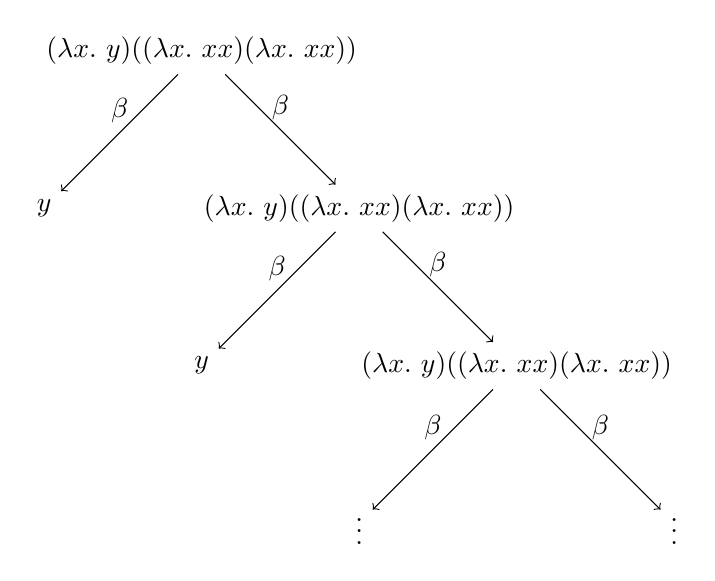
\begin{tikzpicture}
                                \node (o) at (0, 0) {$(\lambda x.\ y)((\lambda x.\ x x)(\lambda x.\ x x))$};
                                \node (ol) at (-2, -2) {$y$};
                                \node (or) at (2, -2) {$(\lambda x.\ y)((\lambda x.\ x x)(\lambda x.\ x x))$};
                                \node (orl) at (0, -4) {$y$};
                                \node (orr) at (4, -4) {$(\lambda x.\ y)((\lambda x.\ x x)(\lambda x.\ x x))$};
                                \node (orrl) at (2, -6) {$\vdots$};
                                \node (orrr) at (6, -6) {$\vdots$};

                                \draw
                                (o) edge[->] node[above]{$\beta$} (ol)
                                (o) edge[->] node[above]{$\beta$} (or)
                                (or) edge[->] node[above]{$\beta$} (orl)
                                (or) edge[->] node[above]{$\beta$} (orr)
                                (orr) edge[->] node[above]{$\beta$} (orrl)
                                (orr) edge[->] node[above]{$\beta$} (orrr);
                            \end{tikzpicture}
                        \end{center}
                \end{itemize}
            \subsubsection*{Reduction Strategies}
                \begin{itemize}
                    \itemsep0em
                    \item \textbf{normal order}
                        \begin{itemize}
                            \itemsep0em
                            \item evaluate the leftmost redex not contained in another redex
                            \item always reduces to a normal form (if one exists)
                            \item can perform computation in unevaluated function bodies (passes unevaluated functions as function arguments)
                        \end{itemize}
                        \begin{align*}
                            & (\violet{(\lambda x y.\ x y x) t} u)((\lambda x y z.\ x ((\lambda x.\ x x) y)) v ((\lambda x.\ x y) w)) \\
                            \to_\beta\ & (\violet{(\lambda y.\ t y t) u})((\lambda x y z.\ x ((\lambda x.\ x x) y)) v ((\lambda x.\ x y) w)) \\
                            \to_\beta\ & (t u t)(\violet{(\lambda x y z.\ x ((\lambda x.\ x x) y)) v} ((\lambda x.\ x y) w)) \\
                            \to_\beta\ & (t u t)(\violet{(\lambda y z.\ v ((\lambda x.\ x x) y)) ((\lambda x.\ x y) w)}) \\
                            \to_\beta\ & (t u t)(\lambda z.\ v (\violet{(\lambda x.\ x x) ((\lambda x.\ x y) w)})) \\
                            \to_\beta\ & (t u t)(\lambda z.\ v (\violet{(\lambda x.\ x y) w}) ((\lambda x.\ x y) w))) \\
                            \to_\beta\ & (t u t)(\lambda z.\ v ((w y) (\violet{(\lambda x.\ x y) w}))) \\
                            \to_\beta\ & (t u t)(\lambda z.\ v ((w y) (w y)))
                        \end{align*}
                    \item \textbf{call by name}
                        \begin{itemize}
                            \itemsep0em
                            \item do not reduce under $\lambda$ (do not reduce inside function bodies that haven't been fully evaluated), and do not evaluate function arguments until you have to
                            \item does not always reduce a term to its normal form
                            \item used in \textit{Haskell} etc.
                        \end{itemize}
                        \begin{align*}
                            & (\violet{(\lambda x y.\ x y x) t} u)((\lambda x y z.\ x ((\lambda x.\ x x) y)) v ((\lambda x.\ x y) w)) \\
                            \to_\beta\ & (\violet{(\lambda y.\ t y t) u})((\lambda x y z.\ x ((\lambda x.\ x x) y)) v ((\lambda x.\ x y) w)) \\
                            \to_\beta\ & (t u t)(\violet{(\lambda x y z.\ x ((\lambda x.\ x x) y)) v} ((\lambda x.\ x y) w)) \\
                            \to_\beta\ & (t u t)(\violet{(\lambda y z.\ v ((\lambda x.\ x x) y)) ((\lambda x.\ x y) w)}) \\
                            \to_\beta\ & (t u t)(\lambda z.\ v ((\lambda x.\ x x) ((\lambda x.\ x y) w)))
                        \end{align*}
                    \item \textbf{call by value}
                        \begin{itemize}
                            \itemsep0em
                            \item do not reduce under $\lambda$, and fully evaluate function arguments before plugging them in
                            \item finds normal forms less often
                            \item most popular strategy, evaluates function arguments only once
                        \end{itemize}
                        \begin{align*}
                            & (\violet{(\lambda x y.\ x y x) t} u)((\lambda x y z.\ x ((\lambda x.\ x x) y)) v ((\lambda x.\ x y) w)) \\
                            \to_\beta\ & (\violet{(\lambda y.\ t y t) u})((\lambda x y z.\ x ((\lambda x.\ x x) y)) v ((\lambda x.\ x y) w)) \\
                            \to_\beta\ & (t u t)((\lambda x y z.\ x ((\lambda x.\ x x) y)) v (\violet{(\lambda x.\ x y) w})) \\
                            \to_\beta\ & (t u t)(\violet{(\lambda x y z.\ x ((\lambda x.\ x x) y)) v} (w y)) \\
                            \to_\beta\ & (t u t)(\violet{(\lambda y z.\ v ((\lambda x.\ x x) y)) (w y)}) \\
                            \to_\beta\ & (t u t)(\lambda z.\ v ((\lambda x.\ x x) (w y))) \\
                        \end{align*}
                \end{itemize}
        \subsection*{4th December 2019 \hfill Lecture}
            \subsubsection*{Definability}
                A partial function $f : \mathbb{N}^n \rightharpoonup \mathbb{N}$ (takes $n$ arguments) is $\lambda$-definable iff there exists a closed $\lambda$-term (no free variables) $\violet{M}$ with the following properties ($\underline{n}$ is the encoding of the natural number $n$ in the $\lambda$-calculus);
                \begin{center}
                    $f(x_1, \dots, x_n) = y \Leftrightarrow \violet{M} \underline{x_1} \dots \underline{x_n} =_\beta y$ and $f(x_1, \dots, x_n) \uparrow \Leftrightarrow \violet{M} \underline{x_1} \dots \underline{x_n}$ has no normal form
                \end{center}
                The Church-Turing Thesis states that if $f$ is computable iff $f$ is register-machine-computable, Turing-machine-computable, or $\lambda$-definable, which means that these models of computation are equivalent.
            \subsubsection*{Constructors}
                Note that the constructors are written in the syntax of \textit{Coq}.
                An ~Inductive~ type can have recursion.
                \begin{itemize}
                    \itemsep0em
                    \item Booleans \hfill ~true, false~
                        \begin{lstlisting}
                            Inductive Bool : Set =
                             | true  : Bool
                             | false : Bool
                        \end{lstlisting}
                        Very simple type, with no underlying recursion - only two values.
                    \item Pairs \hfill ~(a, b)~
                        \begin{lstlisting}
                            Inductive Pair : Set =
                             | pair : elt -> elt -> Pair
                        \end{lstlisting}
                        Despite pairs containing arbitrary data, there is only one way of constructing pairs (~elt~ means element).
                        The notation is that ~(a, b)~ means ~pair a b~.
                    \item Lists \hfill ~[e$_\texttt{1}$, ..., e$_\texttt{n}$]~
                        \begin{lstlisting}
                            Inductive List : Set
                             | nil  : List
                             | cons : elt -> List -> List
                        \end{lstlisting}
                        A list can either be empty (~nil~), or be a head element ~elt~ with a tail ~List~.
                        This is very similar to \textit{Haskell}, so no further explanation \textbf{should} be needed.
                    \item Binary trees \hfill I'm not drawing this out.
                        \begin{lstlisting}
                            Inductive Tree : Set =
                             | leaf   : elt -> Tree
                             | branch : Tree -> elt -> Tree -> Tree
                        \end{lstlisting}
                        A binary tree is either a single ~leaf~, or a ~branch~ which takes in the left subtree, an element, and the right subtree.
                    \item Natural numbers \hfill ~0, 1, 2, ...~
                        \begin{lstlisting}
                            Inductive Nat : Set =
                             | z : Nat
                             | S : Nat -> Nat
                        \end{lstlisting}
                        This is Peano arithmetic, see \textbf{CO142}.
                        The notation is that ~z~ is 0, ~S z~ is 1, ~S (S z)~ is 2, and so on.
                \end{itemize}
            \subsubsection*{Encoding Values}
                \begin{enumerate}[1.]
                    \itemsep0em
                    \item all values are $\lambda$-abstractions, one $\lambda$ per constructor
                    \item the abstraction body is the formal definition of the value
                    \item any non-inductive parameters have to be encoded themselves
                \end{enumerate}
                \begin{itemize}
                    \itemsep0em
                    \item Booleans
                        \smallskip

                        First shorten constructors to $t$ and $f$, giving us a $\lambda$ per constructor.
                        The abstraction bodies are as follows;
                        \begin{align*}
                            \underline{~true~} & = \lambda t f.\ t \\
                            \underline{~false~} & = \lambda t f.\ f
                        \end{align*}
                    \item Pairs
                        \smallskip

                        First shorten constructor to $p$, giving us a single $\lambda$.
                        The abstraction body is as follows;
                        \begin{align*}
                            \underline{~pair a b~} & = \lambda p.\ p\ \underline{a}\ \underline{b}
                        \end{align*}
                    \item Lists
                        \smallskip

                        First shorten constructors to $n$ and $c$, giving us a $\lambda$ per constructor.
                        \begin{align*}
                            \underline{~cons x (cons y (cons z nil))~} & = \lambda c n.\ c\ \underline{x}\ (c\ \underline{y}\ (c\ \underline{z}\ n)
                        \end{align*}
                    \item Binary trees
                        \smallskip

                        Same method as previously, etc.
                        \begin{align*}
                            \underline{~branch (leaf 1) 0 (leaf 2)~} & = \lambda b l.\ b\ (l\ \underline{1})\ \underline{0}\ (l\ \underline{2})
                        \end{align*}
                \end{itemize}
            \subsubsection*{Unpacking}
                Unpacking is the process of using application to remove the $\lambda$s from an encoded value to get the body of the abstraction;
                \begin{align*}
                    (\lambda t f.\ t)\ \violet{t}\ \violet{f} & \to_\beta^* t \\
                    (\lambda p.\ p\ \underline{a}\ \underline{b})\ \violet{p} & \to_\beta^* p\ \underline{a}\ \underline{b} \\
                    (\lambda c n.\ c\ \underline{x}\ (c\ \underline{y}\ (c\ \underline{z}\ n)))\ \violet{c}\ \violet{n} & \to_\beta^* c\ \underline{x}\ (c\ \underline{y}\ (c\ \underline{z}\ n)) \\
                    (\lambda b l.\ b\ (l\ \underline{1})\ \underline{0}\ (l\ \underline{2}))\ \violet{b}\ \violet{l} & \to_\beta^* b\ (l\ \underline{1})\ \underline{0}\ (l\ \underline{2})
                \end{align*}
            \subsubsection*{Encoding Constructors}
                \begin{enumerate}[1.]
                    \itemsep0em
                    \item one $\lambda$ per constructor
                    \item prepend any parameter $\lambda$s to the constructor $\lambda$s
                    \item abstraction body follows the constructor type, with all inductive parameters unpacked
                \end{enumerate}
                \begin{align*}
                    T & = \lambda t f.\ t & ~true~ \\
                    F & = \lambda t f.\ f & ~false~ \\
                    P & = \lambda a b p.\ p\ a\ b & ~pair~ \\
                    N & = \lambda c n.\ n & ~nil~ \\
                    C & = \lambda e l c n.\ c\ e\ (l\ c\ n) & ~cons~
                    \intertext{note how the ~cons~ constructor has $(l\ c\ n)$, as the inductive parameter must be unpacked}
                    L & = \lambda e b l.\ l\ e & ~leaf~ \\
                    B & = \lambda t_1 e t_2 b l.\ b\ (t_1\ b\ l)\ e\ (t_2\ b\ l) & ~branch~
                \end{align*}
                A proof of this working for ~cons~ is as follows (note the use of $\to_\beta^*$ to denote multiple steps - important for exam);
                \begin{align*}
                    & C\ \underline{x}\ (C\ \underline{y}\ N) \\
                    \triangleq\ & C\ \underline{x}\ ((\lambda e l c n.\ c\ e\ (l\ c\ n))\ \underline{y}\ N) \\
                    \to_\beta^*\ & C\ \underline{x}\ (\lambda c n.\ c\ \underline{y}\ (N\ c\ n)) \\
                    \triangleq\ & C\ \underline{x}\ (\lambda c n.\ c\ \underline{y}\ ((\lambda c n.\ n)\ c\ n)) \\
                    \to_\beta^*\ & C\ \underline{x}\ (\lambda c n.\ c\ \underline{y}\ n) \\
                    \triangleq\ & (\lambda e l c n.\ c\ e\ (l\ c\ n))\ \underline{x}\ (\lambda c n.\ c\ \underline{y}\ n) \\
                    \to_\beta^*\ & (\lambda c n.\ c\ \underline{x}\ ((\lambda c n.\ c\ \underline{y}\ n)\ c\ n)) \\
                    \to_\beta^*\ & \lambda c n.\ c\ \underline{x}\ (c\ \underline{y}\ n)
                \end{align*}
            \subsubsection*{Encoding Operations}
                The idea is to manipulate the encoding body by inserting a function in place of the constructor.
                For example, with a pair $\lambda p.\ p\ a\ b$, if we want the first element, we want $a$, otherwise we want $b$ if we want the second element.
                \begin{align*}
                    Fst & = \lambda p.\ p\ (\lambda a b.\ a) \\
                    Snd & = \lambda p.\ p\ (\lambda a b.\ b)
                \end{align*}
                For example;
                \begin{align*}
                    & Fst (\lambda p.\ p\ \underline{0}\ \underline{1}) \\
                    \triangleq\ & (\lambda p.\ p\ (\lambda a b.\ a)) (\lambda p.\ p\ \underline{0}\ \underline{1}) \\
                    \to_\beta\ & (\lambda p.\ p\ \underline{0}\ \underline{1}) (\lambda a b.\ a) \\
                    \to_\beta\ & (\lambda a b.\ a)\ \underline{0}\ \underline{1} \\
                    \to_\beta^*\ & \underline{0}
                \end{align*}
                Similarly for the head and tail of a list, we have;
                \begin{align*}
                    Hd & = \lambda l.\ l\ (\lambda e l.\ e)\ \_ \\
                    Tl & = \lambda l.\ l\ (\lambda e l.\ (\lambda c n.\ l))\ \_
                \end{align*}
                Note the use of the $\_$, since the constructor for a list has two parameters, we want to discard the $n$ (~nil~) constructor, since it doesn't make sense to use this on the empty list.
                It's also important to note that we also need the additional $c n$ parameters for the tail to pack the list.
                However, now we have $Hd\ N =_\beta Tl\ N =_\beta \_$, since both those functions are total (in terms of $\lambda$-definability).
                Therefore this must be adjusted to not have a normal form.
            \subsubsection*{Constructor Recognisers}
                In order to do this, we have to employ constructor recognisers, which are mechanisms designed to recognise the lead constructor then branch using that mechanism.
                A use case for this is for $Hd$ to recognise whether it's being applied to the empty list (and thus diverge), or to proceed otherwise.
                \begin{align*}
                    isNil & = \lambda l.\ l\ (\lambda e l.\ \underline{false})\ (\underline{true}) \\
                    isCons & = \lambda l.\ l\ (\lambda e l.\ \underline{true})\ (\underline{false})
                    \intertext{this can now be used for branching as follows;}
                    ifNil & = \lambda x y l.\ l\ (\lambda e l.\ y)\ x
                    \intertext{give it some term without a normal form (diverges) as follows;}
                    D & = (\lambda x.\ x x)(\lambda x.\ x x)
                    \intertext{we can now create partial functions that can diverge (which is the correct use)}
                    PHd & = ifNil\ D\ Hd \\
                    PTl & = ifNil\ D\ Tl
                \end{align*}
            \subsubsection*{Encoding Natural Numbers}
                The Church numerals are encoded as follows;
                \begin{align*}
                    \underline{0} & = \lambda s z.\ z \\
                    \underline{1} & = \lambda s z.\ s\ z \\
                    \underline{2} & = \lambda s z.\ s\ (s\ z) \\
                    \underline{3} & = \lambda s z.\ s\ (s\ (s\ z)) \\
                    & \cdots \\
                    \underline{n} & = \lambda s z.\ \underbrace{s\ (\dots\ (s}_n\ z)\ \dots\ )
                \end{align*}
                In order to encode addition of two natural numbers, $m$ and $n$, we want;
                \begin{align*}
                    \underline{m} =\ & \lambda s z.\ \underbrace{s\ (\dots(s}_m\ \red{z})\dots) \\
                    \underline{n} =\ & \lambda s z.\ \blue{\underbrace{s\ (\dots(s}_n\ z)\dots)} \\
                    plus\ \underline{m}\ \underline{n} =_\beta\ & \lambda s z.\ \underbrace{s\ (\dots(s}_{m + n}\ z)\dots)
                \end{align*}
                Ideally, we want to substitute the \blue{blue} part of $\underline{n}$ into the \red{red} part of $\underline{m}$.
                To achieve this, we can do the following steps;
                \begin{enumerate}[1.]
                    \itemsep0em
                    \item unpack to obtain the body of $\underline{n}$ \hfill $\underline{n}\ s\ z =_\beta \underbrace{s(\dots(s}_n\ z)\dots)$
                    \item unpack $\underline{m}$ with the unpacked $\underline{n}$ in place of $z$ \hfill $\underline{m}\ s\ (\underline{n}\ s\ z) =_\beta \underbrace{s(\dots(s}_{m + n}\ z)\dots)$
                    \item pack into a Church numeral \hfill $\lambda s z.\ \underline{m}\ s\ (\underline{n}\ s\ z) =_\beta \underline{m + n}$
                    \item make this into a function that takes $m$ and $n$ \hfill $plus \triangleq \lambda m n s z.\ m\ s\ (n\ s\ z)$
                \end{enumerate}
        \subsection*{5th December 2019 \hfill Lecture}
            \subsubsection*{Multiplication}
                For short, let us define $n$ applications of $s$ as follows; $s^n$, allowing for the following;
                \begin{align*}
                    \underline{m} & = \lambda s z.\ s^m\ z \\
                    \underline{n} & = \lambda s z.\ s^n\ z \\
                    \underline{m + n} & = \lambda s z.\ s^{m + n}\ z
                \end{align*}
                To encode multiplication, we only partially unpack $\underline{n}$, using $(n\ s)$, instead of $(n\ s\ z)$ in place of $s$ in $\underline{m}$ (similar strategy to what we did for addition).
                \begin{align*}
                    m\ (n\ s) =\ & (\lambda s z.\ s^m\ z)(n\ s) \\
                    =\ & (\lambda s z.\ s^m\ z)(\lambda z.\ s^n\ z) \\
                    =_\beta\ & (\lambda z.\ (\lambda z.\ s^n\ z)^m\ z) \\
                    \to_\beta\ & (\lambda z.\ (\lambda z.\ s^n\ z)^{m - 1}\ (s^n\ z)) \\
                    \to_\beta\ & (\lambda z.\ (\lambda z.\ s^n\ z)^{m - 2}\ (s^{2 \cdot n}\ z)) \\
                    \to_\beta^*\ & (\lambda z.\ s^{m \cdot n}\ z) \\
                    \underline{m \cdot n} =\ & \lambda s z.\ s^{m \cdot n}\ z \\
                    =\ & \lambda s.\ m\ (n\ s) \\
                    mult \triangleq\ & \lambda m n s.\ m\ (n\ s)
                \end{align*}
            \subsubsection*{Combinators}
                \textbf{Combinators} are closed $\lambda$-terms.
                The most important ones are $I$, $K$, and $S$;\
                \begin{align*}
                    I & \triangleq \lambda x.\ x & \text{identity} \\
                    I & : \alpha \to \alpha \\
                    K & \triangleq \lambda x y.\ x & \text{true / selector} \\
                    K & : \alpha \to \beta \to \alpha \\
                    S & \triangleq \lambda x y z.\ x z (y z) \\
                    S & : \underbrace{(\alpha \to \beta \to \gamma)}_x \to \underbrace{(\alpha \to \beta)}_y \to \underbrace{\alpha}_z \to \gamma
                \end{align*}
                All of the $\lambda$-calculus we have covered can be done with the $SKI$ combinators ($I$ is also $SKK$).
            \subsubsection*{Recursion}
                For an example of recursion, we will be using the factorial.
                \begin{align*}
                    fact\ n \triangleq\ & \text{if } (n = 0) \text{ then } 1 \text{ else } n \cdot fact\ (n - 1) \\
                    ifz\ \underline{n}\ x\ y =_\beta\ & \begin{cases}
                        x & n = 0 \\
                        y & n > 0
                    \end{cases} \\
                    fact =_\beta\ & \lambda n.\ ifz\ n\ \underline{1}\ (mult\ n\ (fact\ (pred\ n))) \\
                    =_\beta\ & \underbrace{(\lambda f.\ \lambda n.\ ifz\ n\ \underline{1}\ (mult\ n\ (f\ (pred\ n))))}_F\ fact
                \end{align*}
                In mathematics, if $f(x) = x$, then $x$ is a \textbf{fixpoint} of $f$.
                As such, we have $fact$ being a fixpoint of $F$.
                \begin{align*}
                    Y \triangleq\ & \lambda f.\ (\lambda x.\ f\ (x x)) (\lambda x.\ f\ (x x)) \\
                    Y\ f \triangleq\ & (\lambda f.\ (\lambda x.\ f\ (x x)) (\lambda x.\ f\ (x x)))\ f \\
                    \to_\beta\ & (\lambda x.\ f\ (x x)) (\lambda x.\ f\ (x x)) \\
                    \to_\beta\ & f\ ((\lambda x.\ f\ (x x))\ (\lambda x.\ f\ (x x))) \\
                    =_\beta\ & f\ (Y\ f)
                \end{align*}
                Therefore, $Y\ f$ is a fixpoint of $f$.
                The $Y$ combinator is the \textbf{fixpoint operator}.
                As such, we can define the factorial as;
                \begin{center}
                    $fact \triangleq Y\ (\lambda f.\ \lambda n.\ ifz\ n\ \underline{1}\ (mult\ n\ (f\ (pred\ n))))$
                \end{center}
            \subsubsection*{$\eta$-equivalence}
                $(\lambda x.\ f\ x) \neq_\beta f$, despite always having the case $(\lambda x.\ f\ x)\ M =_\beta f\ M$.
                However, there is no way to capture this with $\beta$-reduction.
                This can be captured with the following rule;
                \begin{center}
                        \axiom{$x \notin \text{FV}(\violet{M})$}
                    \unary{$\lambda x.\ \violet{M}\ x =_\eta \violet{M}$}
                    \dproof
                \end{center}
\end{document}
